\chapter{Моделирование МКАД}\label{sec:ch5}
В данном разделе на модельных данных проверим гипотезу о возможности повышения пропускной способности автомагистрали за счет адаптивного управления её въездами на примере МКАД.
Для проверки данной гипотезы на реальных данных у нас недостаточно информации с дорожных датчиков на въезде на МКАД.
В разделе также приводится процедура построения математической модели МКАД с помощью данных топологии GPS-навигатора, обоснование построение модельного потока на въезде и принцип принятия решения автомобилистами о съезде с автомагистрали.

\section{Построение модели МКАД}
\label{sec:MCAR_model}
Модель транспортной сети в данной работе представляет из себя связанный ориентированный граф \(\mathbf{G}\).
Данный граф строится на основе топологии МКАД и прилегающих к нему дорог.
При построении графа вручную размечаются основные ребра-въезды на автомагистраль и ребра-съезды с автомагистрали.
Причем разметка въездов разделяет их на два типа~--- въезды с магистралей, направленных в Москву, и с магистралей, направленных из Москвы.
Это нужно ввиду того, что пиковый поток на этих двух типах въездов приходится на разное время суток.

Поскольку в топологии не выделены сегменты, отвечающие за сам МКАД, но указаны координаты каждого ребра, то выделение автомагистрали проводится следующим образом:
\begin{enumerate}
  \item Выбирается один сегмент \(i\) на автомагистрали; так как координаты начала и конца сегмента известны, то можем представить его как вектор \(\mathbf{i}\).
  \item Ищутся все сегменты топологии, идущие после него, и считается их векторное представление. Обозначим множество этих векторов через \(\mathbf{S}\).
  \item \(\forall \mathbf{j} \in \mathbf{S}\)~--- рассчитываем угол между векторами \((\mathbf{i}; \mathbf{j})\) и выбираем сегмент с наименьшим углом как продолжение магистрали \(\mathbf{i'}\).
  \item Возвращаемся к пункту 1 с \(\mathbf{i} = \mathbf{i'}\), пока не вернулись в исходный сегмент (для МКАД) или не достигнем ее конца (в этом случае требуется задать сегмент~--- конец автомагистрали).
\end{enumerate}
Данная процедура значительно уменьшает объемы ручной работы для формирования графа \(\mathbf{G}\).
Однако она все же допускает ошибки и требуется формирование небольшого списка сегментов топологии, точно не являющихся искомой автомагистралью.
В данной работе этот список состоит из 14 сегментов.
Все еще требуется вручную разметить основные въезды и съезды с автомагистрали, однако можно проигнорировать незначительные, т.е. съезды на небольшие прилегающие дороги и въезды на них, поток на которых пренебрежимо мал для целей этой работы.

В результате работы по данному алгоритму получен связный ориентированный граф \(\mathbf{G}\) одной из сторон МКАД со всеми необходимыми въездами и съездами.

\section{Генерация синтетических данных на въездах}
\label{sec:MCAR_data}
Ввиду отсутствия открытых источников данных с дорожных датчиков на въездах требуется сгенерировать реалистичный поток автомобилей синтетически.
По информации от ЦОДД~\cite{CODD_MKAD} по всему МКАД за сутки проезжает 1,36 миллионов автомобилей (т.е. приблизительно 680 тысяч АТС по одной стороне), а по имеющимся данным с дорожных датчиков пиковый поток АТС на въезде составляет 60 АТС/мин.
Пример данных с дорожных датчиков показан на рис.~\ref{fig:Detector_example}.
\begin{figure}[ht]
    \centerfloat{
        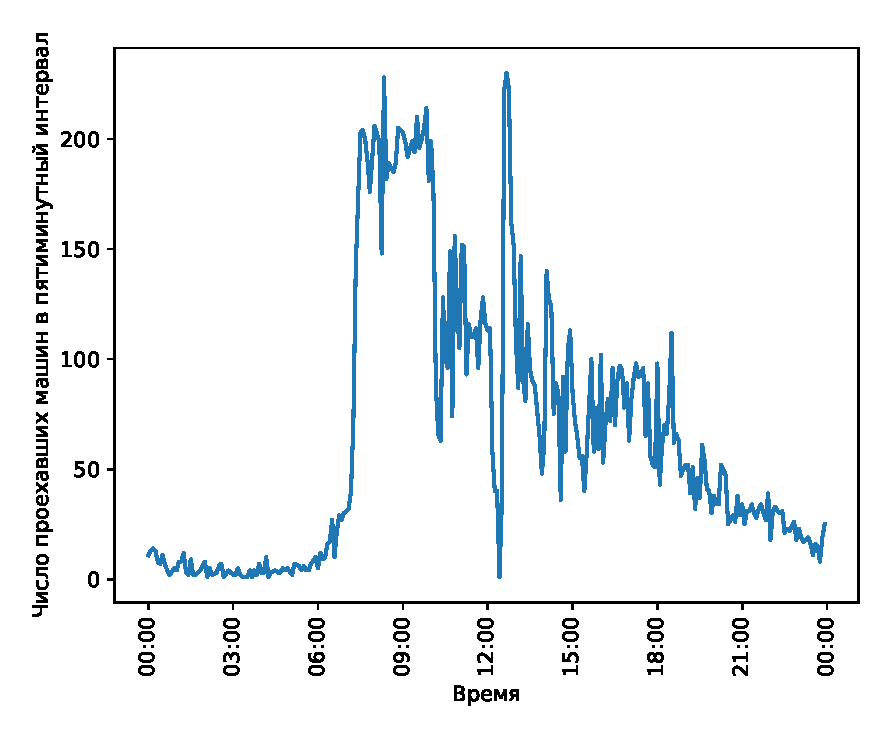
\includegraphics[width=1.0\linewidth]{Detector.eps}
    }
    \caption{Данные с дорожного датчика за один день. Пиковая нагрузка 45 АТС/мин в 8:20.}
    \label{fig:Detector_example}
\end{figure}

Таким образом, в экспериментах функции входного потока на въездах строились так, чтобы походить на данные с реального дорожного детектора и соответствовали информации о пиковой (или средней, если это требовалось) нагрузке на въезде и числу проезжающих по автомагистрали за день АТС.

Как говорилось выше, все въезды также вручную были разделены на два класса:
\begin{enumerate}
  \item Въезды с магистралей по направлению из Москвы, на которых поток АТС нарастает ближе к вечеру.
  \item Въезды с магистралей по направлению в Москву, на которых поток АТС нарастает утром и спадает к вечеру.
\end{enumerate}


\section{Описание данных}
\label{sec::data}
В разделе проводится моделирование внешней стороны Московской кольцевой автомобильной дороги~(МКАД), рис.~\ref{fig:MCAR_map}.
Для построения графа использовалась топология, взятая у компании Яндекс в 2014 г.
Полученная топология, а также увеличенный участок МКАД со съездами и въездами изображены на рис.~\ref{fig:MCAR_topology}.

\begin{figure}[ht]
    \centerfloat{
        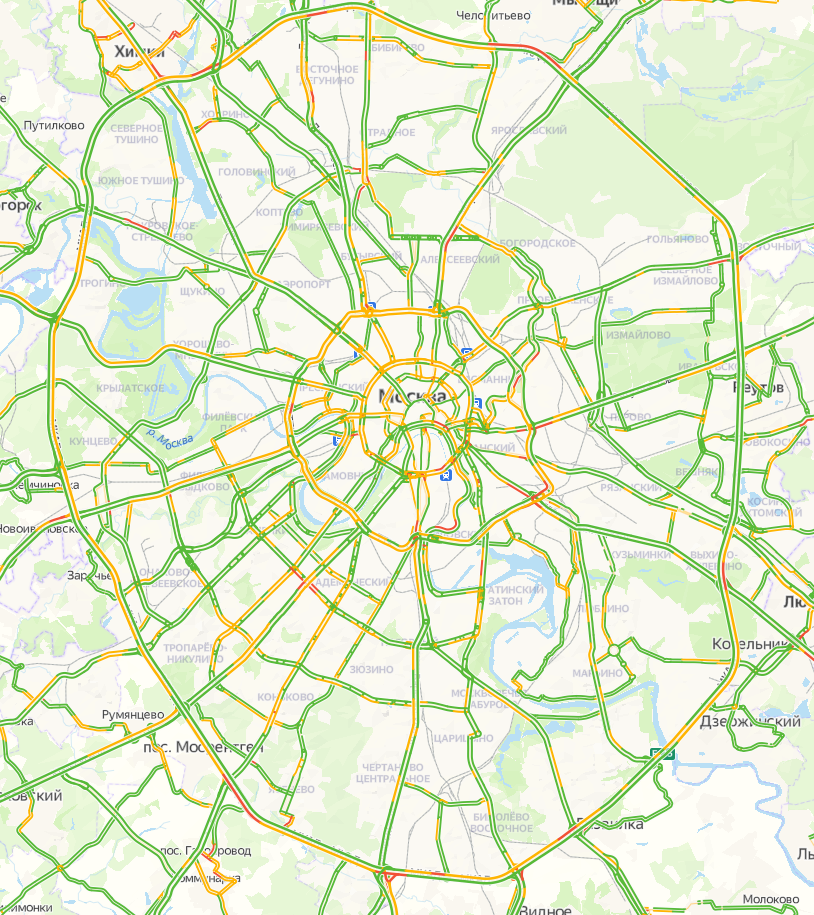
\includegraphics[width=1.0\linewidth]{YandexMap2.png}
    }
    \caption{Типичные пробки по понедельникам в 18:15 на основе статистики сервиса «Яндекс-пробки» транспортной сети Москвы и МКАД, в частности по состоянию на 16.05.21.}
    \label{fig:MCAR_map}
\end{figure}

\begin{figure}[ht]
    \begin{minipage}[b][][b]{0.7045\textwidth}
        \centering
        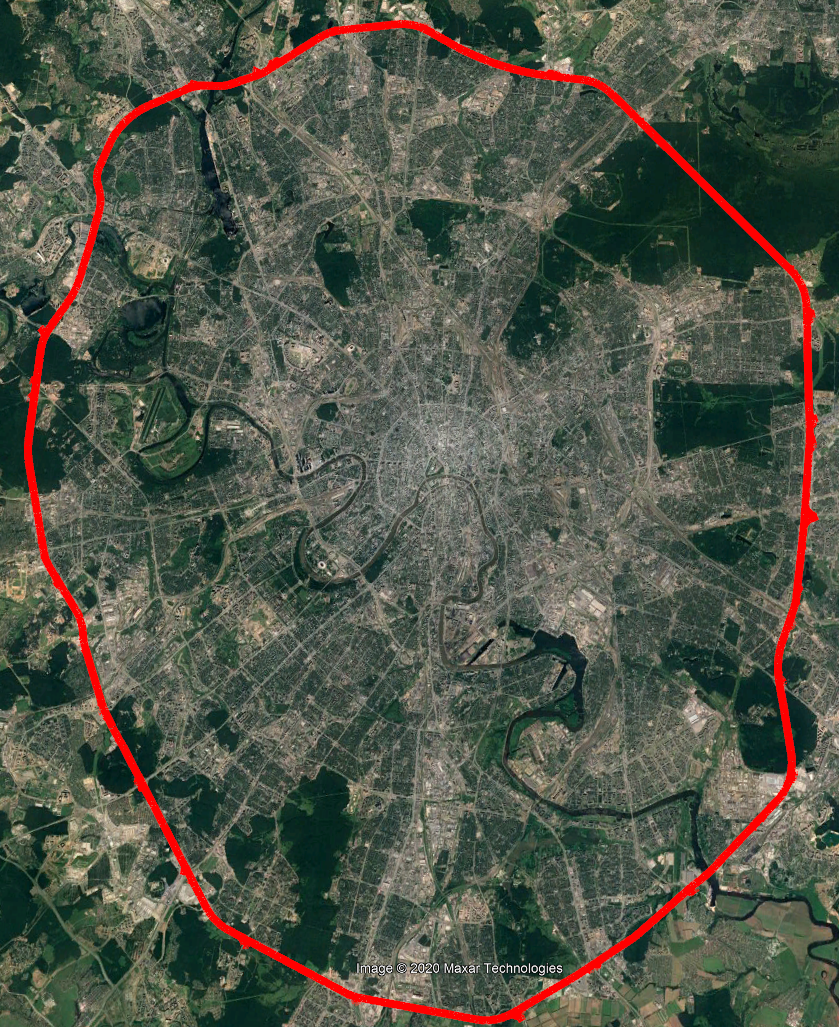
\includegraphics[width=1\linewidth]{YandexMCAR_topology.png} \\ а)
    \end{minipage}
    \hfill
    \begin{minipage}[b][][b]{0.2755\textwidth}
        \centering
        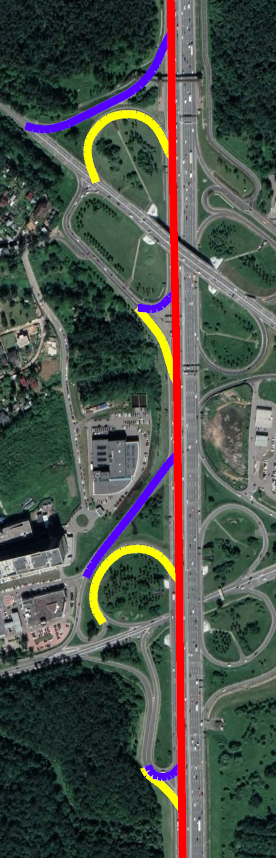
\includegraphics[width=1\linewidth]{YandexMCAR_topology_enter.png} \\ б)
    \end{minipage}

    \caption{а) Вид рассчетного графа МКАД, полученного с помощью топологии компании Яндекс, б) Конфигурация въездов и съездов с МКАД в полученном на основе топологии компании Яндекс графе. Красная линия~--- МКАД, желтая~--- въезды на магистраль, синяя~--- съезды с нее.}
    \label{fig:MCAR_topology}
\end{figure}

В данном разделе во всех экспериментах использовалось несколько фундаментальных диаграмм поток-плотность, полученных анализом реальных данных с дорожных датчиков за 2012 г.
Бралось всего несколько фундаментальных диаграмм эмпирическим образом распределенных между участками МКАД с целью проверки работоспособности модели в ситуации существенно недостаточных для построения всех диаграмм данных.
В следующих разделах будет показан полный эксперимент на основе всех фундаментальных диаграмм поток-плотность для всех сегментов транспортной сети.

\section{Вычислительные эксперименты}
\label{sec::experiments}
Проведены следующие группы вычислительных экспериментов:
\begin{enumerate}
  \item Эксперименты со средней, но продолжительной, пиковой загрузкой на въезды с проверкой эффекта от динамического ограничения входного потока в зависимости от состояния автомагистрали.
  \item Эксперименты с высокой, но непродолжительной, пиковой загрузкой въездов (что более соответствует данным от ЦОДД) с проверкой эффекта от динамического ограничения входного потока в зависимости от состояния автомагистрали.
  \item Эксперименты с длинными въездами с высокой, но непродолжительной, пиковой загрузкой въездов с проверкой эффекта от динамического ограничения входного потока в зависимости от состояния автомагистрали. В данной группе экспериментов максимальная длина очереди на въездах на МКАД увеличена для расчетов времени ожидания на въезде на магистраль без управления въездами и с ним.
\end{enumerate}

В связи с отсутствием реальных данных о числе покидающих автомагистраль транспортных средств в каждый момент времени считаем эту долю фиксированной и выбранной из следующих соображений:
\begin{enumerate}
  \item проезжать более половины МКАД в одну сторону неосмысленно так как в данном случае можно поехать в другую сторону,
  \item на половине МКАД в рассматриваемой модели 32 съезда.
\end{enumerate}
Таким образом, если \(x\)~--- доля съезжающих на каждом съезде АТС, то величина \((1-x)^{30}\) должна быть мала. В экспериментах используется величина \(x = 12\%\).

В каждой группе экспериментов также проводится моделирование ситуации установки светофора на въездах на автомагистраль.
В таком случае алгоритм ограничения входного потока на МКАД выглядит следующим образом:
\begin{itemize}
  \item Для каждого сегмента автомагистрали по направлению движения АТС после рассматриваемого въезда посчитаем плотность автомобилей \(\rho\) на ней.
  \item В зависимости от величины \(\rho_{\text{opt}} - \rho$, где $\rho_{\text{opt}}\)~--- плотность, при которой достигается максимальный поток на рассматриваемом сегменте автомагистрали, входной поток ограничивается на \(l<l_{\text{max}}\) процентов.
  \item Ограничения для каждого из сегментов складываются и получается результирующее понижение входного потока АТС.
\end{itemize}

Важной характеристикой моделируемой системы считаем временные потери на проезд по транспортной сети относительно пустой автомагистрали, т.е. автомагистрали, по которой возможно движение АТС с максимально допустимой скоростью.
Каждую минуту рассчитывается среднее продвижение каждого автомобиля в модели и сравнивается с расстоянием, которое он мог бы преодолеть по пустой магистрали.
Это преобразуется в график временных потерь, который трактуется как время простоя автомобиля в транспортной сети за минуту.

\subsection{Эксперименты со средней загрузкой}
\label{sec:ch5/average}
В данной группе экспериментов въезды считаются однополосными и функции входного потока изображены на рис.~\ref{fig:MCAR_flow_low_3h}.
В данном случае есть два типа въездов на автомагистраль~--- с утренней и вечерней пиковыми загрузками в течение трех часов.
\begin{figure}[ht]
    \begin{minipage}[b][][b]{0.49\textwidth}
        \centering
        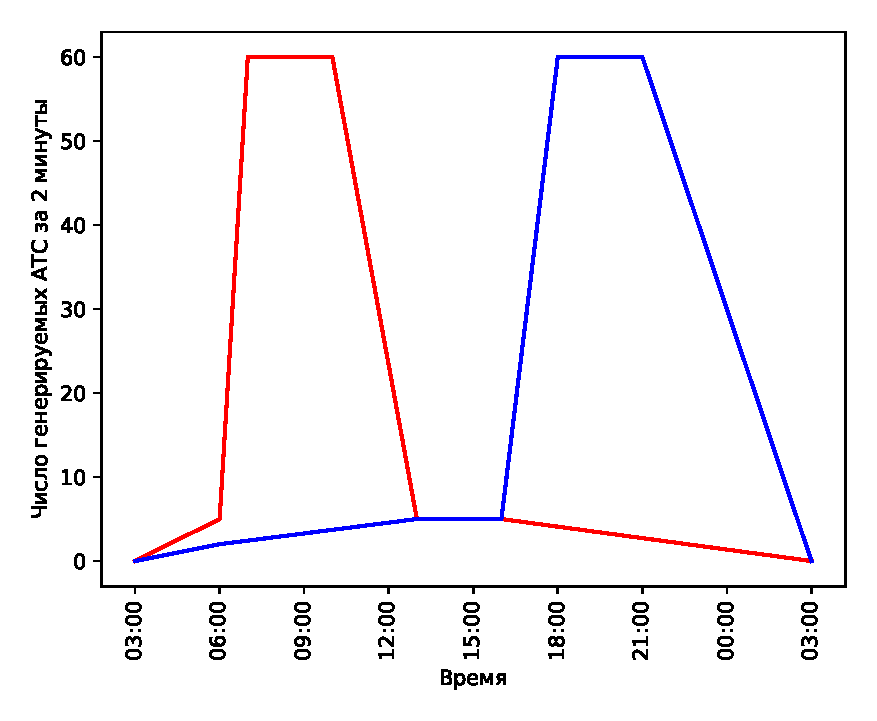
\includegraphics[width=1\linewidth]{MCAR_full_woenters_12_two_types_60_24h_3hmax_Enters_generators.eps}
        \caption{Графики загрузки двух типов въездов~--- с утренней и вечерней пиковыми загрузками в эксперименте со средней загрузкой.}
        \label{fig:MCAR_flow_low_3h}
    \end{minipage}
    \hfill
    \begin{minipage}[b][][b]{0.49\textwidth}
        \centering
        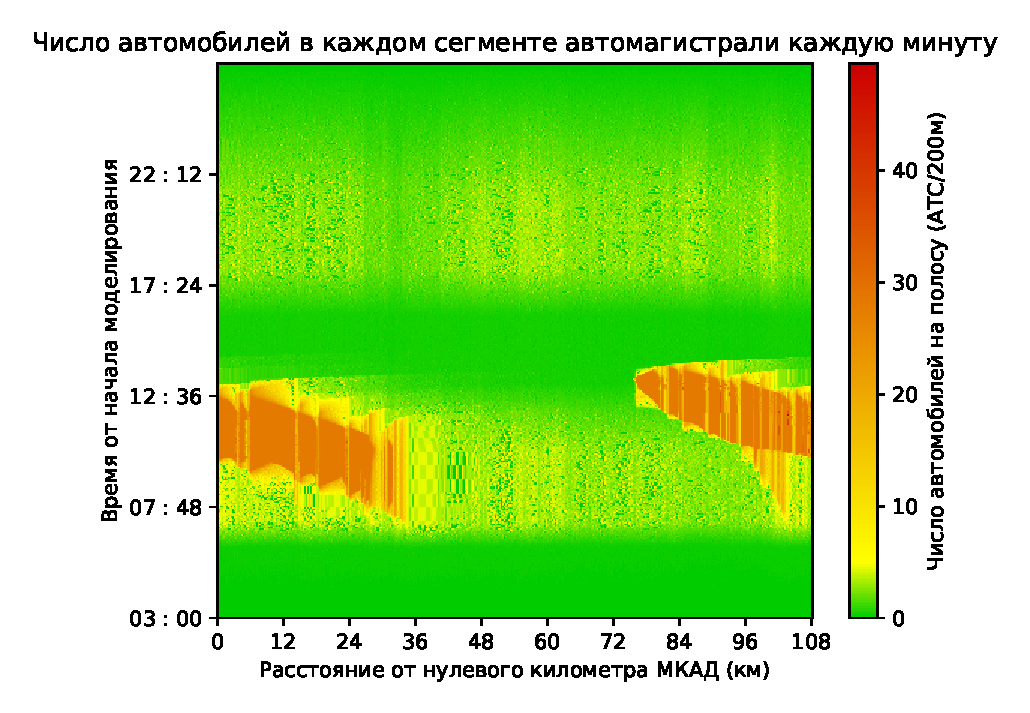
\includegraphics[width=1\linewidth]{MCAR_full_woenters_12_two_types_60_24h_3hmax.eps}
        \caption{Количество автомобилей на полосе в модели транспортной сети за день в эксперименте со средней загрузкой.}
        \label{fig:MCAR_heatmap_low_3h}
    \end{minipage}
\end{figure}

\subsection{Эксперимент без управления въездами}
Результаты моделирования автомагистрали при такой конфигурации въездов представлены на рис.~\ref{fig:MCAR_heatmap_low_3h}.
Число реально въехавших автомобилей и количество проехавших за день по транспортной сети АТС изображены на рис.~\ref{fig:MCAR_entered_low_3h}.
График временных потерь~- на рис.~\ref{fig:MCAR_timeloss_low_3h}.

Видно, что при такой конфигурации входных потоков заторы возникают всего в нескольких местах и потом со временем распространяются по автомагистрали.
Так как пробки успевают исчезнуть к вечеру, то МКАД не останавливается полностью, хотя при меньшей доли съезжающих автомобилей это произойдет.
\begin{figure}[ht]
    \begin{minipage}[b][][b]{0.49\textwidth}
        \centering
        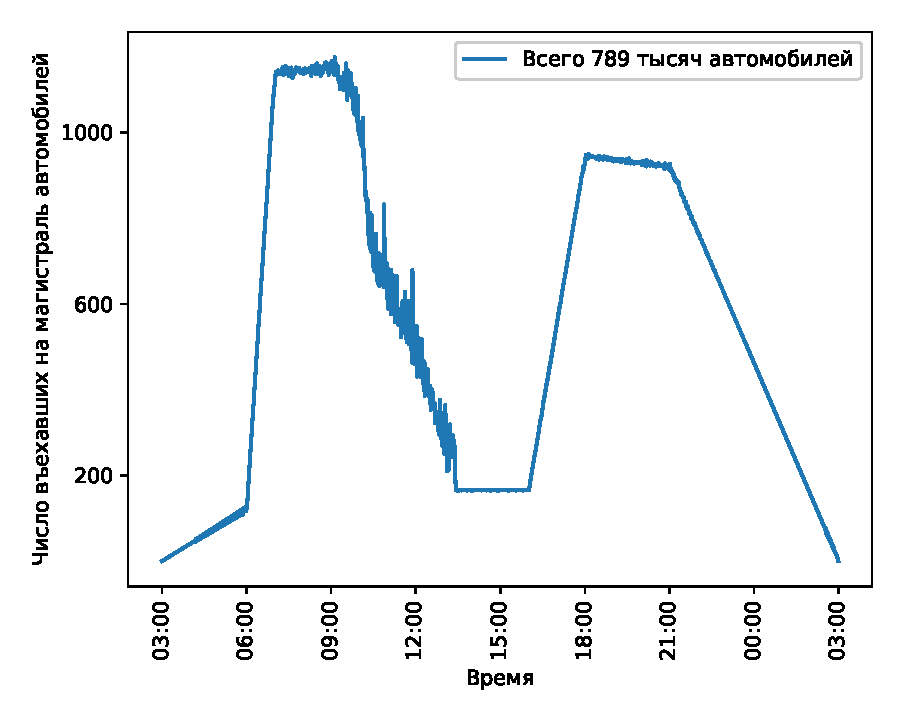
\includegraphics[width=1\linewidth]{MCAR_full_woenters_12_two_types_60_24h_3hmax_Entered.eps}
        \caption{График суммарно въехавшего на автомагистраль со всех въездов числа автомобилей в эксперименте со средней загрузкой.}
        \label{fig:MCAR_entered_low_3h}
    \end{minipage}
    \hfill
    \begin{minipage}[b][][b]{0.49\textwidth}
        \centering
        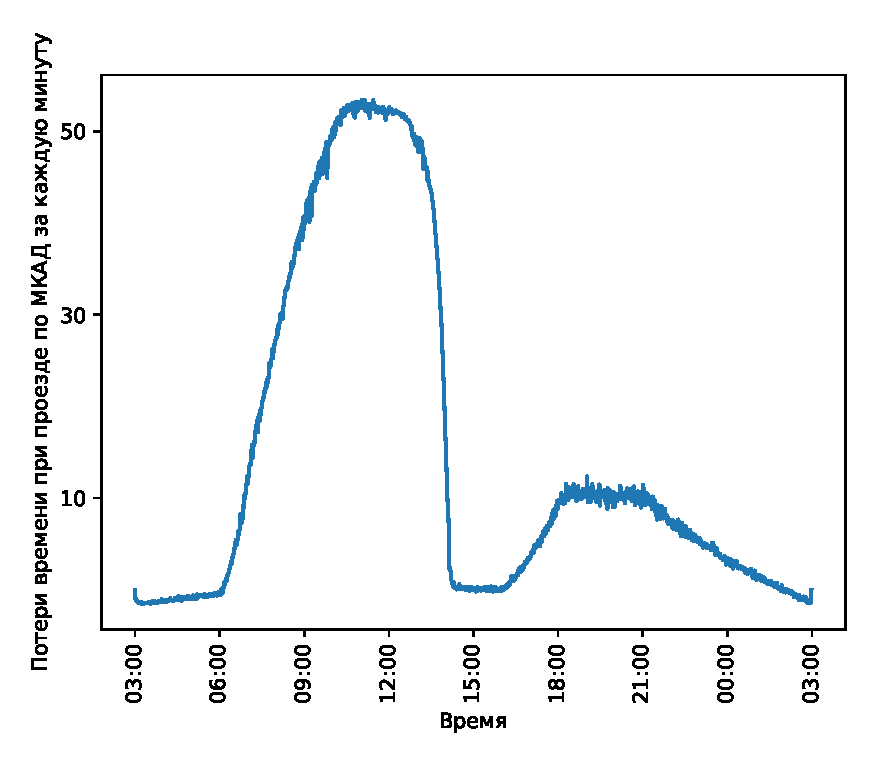
\includegraphics[width=1\linewidth]{MCAR_full_woenters_12_two_types_60_24h_3hmax_Time_to_pass.eps}
        \caption{Временные потери на проезд по автомагистрали в эксперименте со средней загрузкой.}
        \label{fig:MCAR_timeloss_low_3h}
    \end{minipage}
\end{figure}


\subsection{Эксперимент с управлением въездами}
Промоделируем ситуацию, в которой при увеличении потока на автомагистрали будем ограничивать поток с ближайших въездов на автомагистраль искусственно, например с помощью светофора.
В данном эксперименте можем перекрывать въезд вплоть до 80\% в зависимости от плотности автомобилей на магистрали.
Результаты моделирования при такой конфигурации въездов представлены на рис.~\ref{fig:MCAR_heatmap_low_3h_handcontrol}.
Число реально въехавших автомобилей и количество проехавших за день по транспортной сети АТС изображены на рис.~\ref{fig:MCAR_entered_low_3h_handcontrol}.
График временных потерь проезда по всей автомагистрали представлен на рис.~\ref{fig:MCAR_timeloss_low_3h_handcontrol}.
\begin{figure}[ht]
    \centerfloat{
        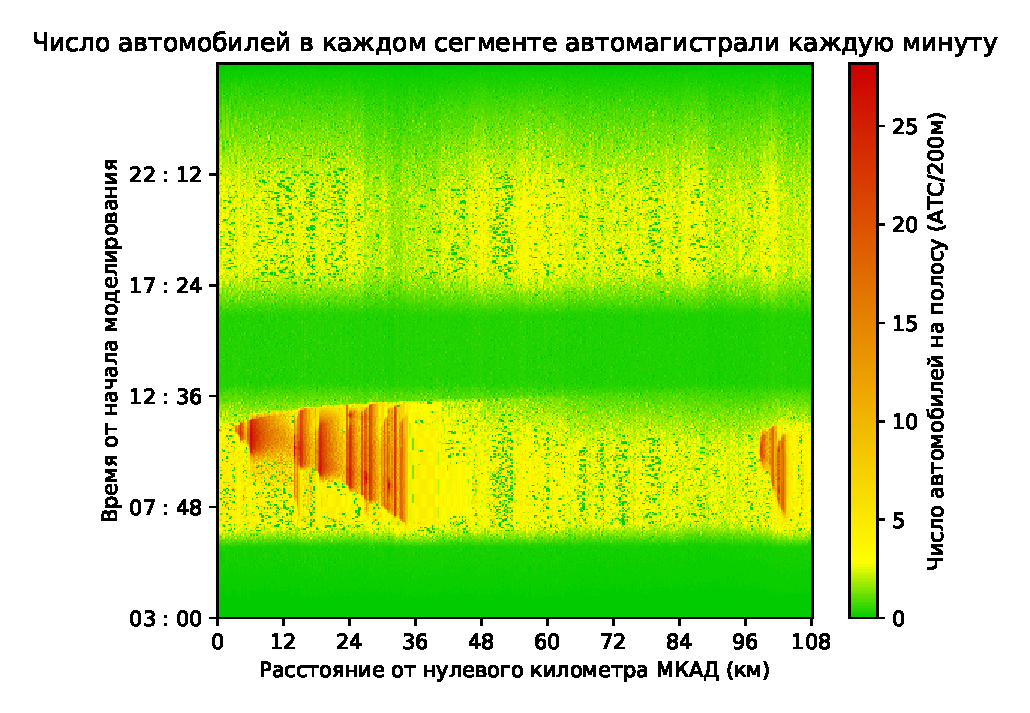
\includegraphics[width=0.8\linewidth]{MCAR_full_woenters_12_two_types_60_24h_3hmax_handcontrol.eps}
    }
    \caption{Количество автомобилей на полосе в модели транспортной сети за день в эксперименте со средней загрузкой с управлением въездами.}
    \label{fig:MCAR_heatmap_low_3h_handcontrol}
\end{figure}

\begin{figure}[ht]
    \begin{minipage}[b][][b]{0.49\textwidth}
        \centering
        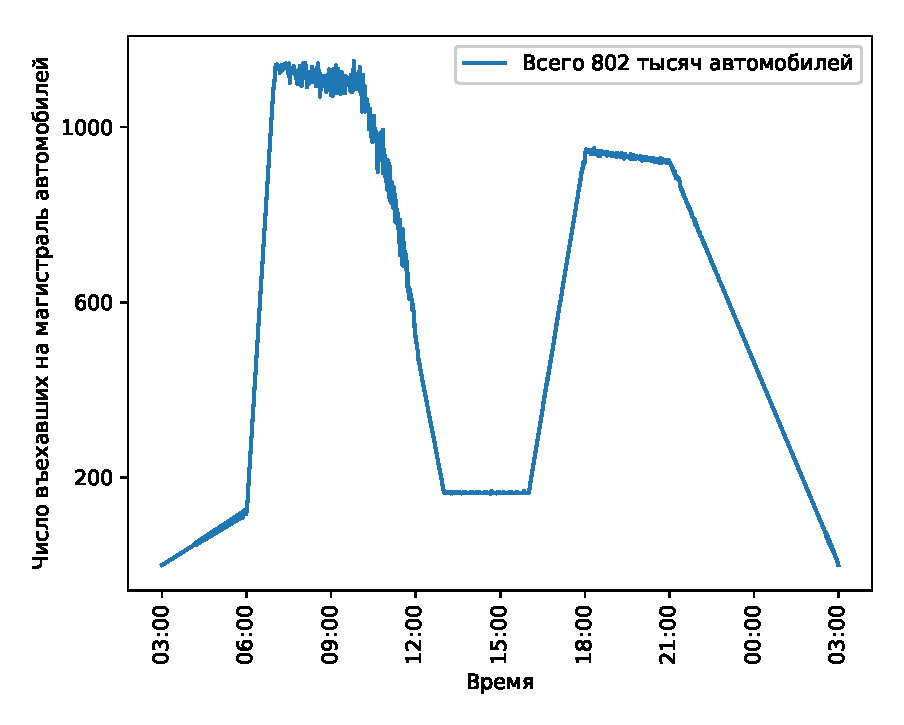
\includegraphics[width=1\linewidth]{MCAR_full_woenters_12_two_types_60_24h_3hmax_handcontrol_Entered.eps}
        \caption{График суммарно въехавшего на автомагистраль со всех въездов числа автомобилей в эксперименте со средней загрузкой с управлением въездами.}
        \label{fig:MCAR_entered_low_3h_handcontrol}
    \end{minipage}
    \hfill
    \begin{minipage}[b][][b]{0.49\textwidth}
        \centering
        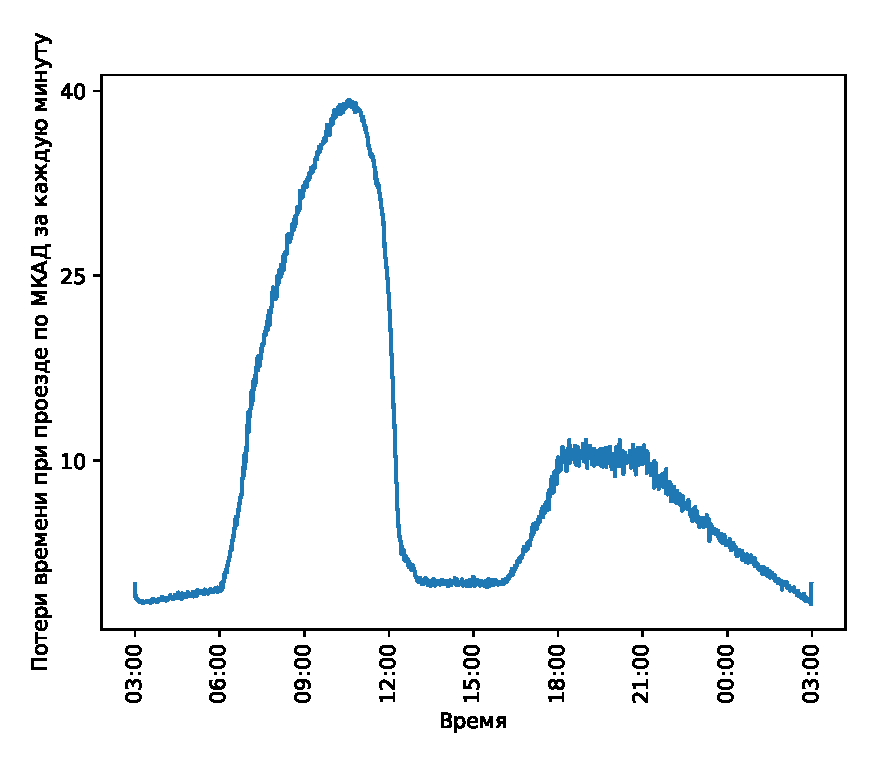
\includegraphics[width=1\linewidth]{MCAR_full_woenters_12_two_types_60_24h_3hmax_handcontrol_Time_to_pass.eps}
        \caption{Временные потери на проезд по автомагистрали в эксперименте со средней загрузкой с управлением въездами.}
        \label{fig:MCAR_timeloss_low_3h_handcontrol}
    \end{minipage}
\end{figure}

На графиках видно уменьшение времени затора на МКАД, а также небольшое увеличение числа проехавших автомобилей.
Однако временные потери на проезд по автомагистрали значительно снизились.
Интегральная разность между графиками временных потерь на рис.~\ref{fig:MCAR_timeloss_low_3h}~и~\ref{fig:MCAR_timeloss_low_3h_handcontrol} составляет около $4,5$ минут.


\section{Эксперименты с высокой загрузкой}
\label{sec:ch5/hight}
В данной группе экспериментов въезды считаются двухполосными и функции входного потока изображены на рис.~\ref{fig:MCAR_flow_hight_3h}.
В данном случае есть два типа въездов на автомагистраль~--- с утренней и вечерней пиковыми загрузками в течение трех часов.
\begin{figure}[ht]
    \begin{minipage}[b][][b]{0.49\textwidth}
        \centering
        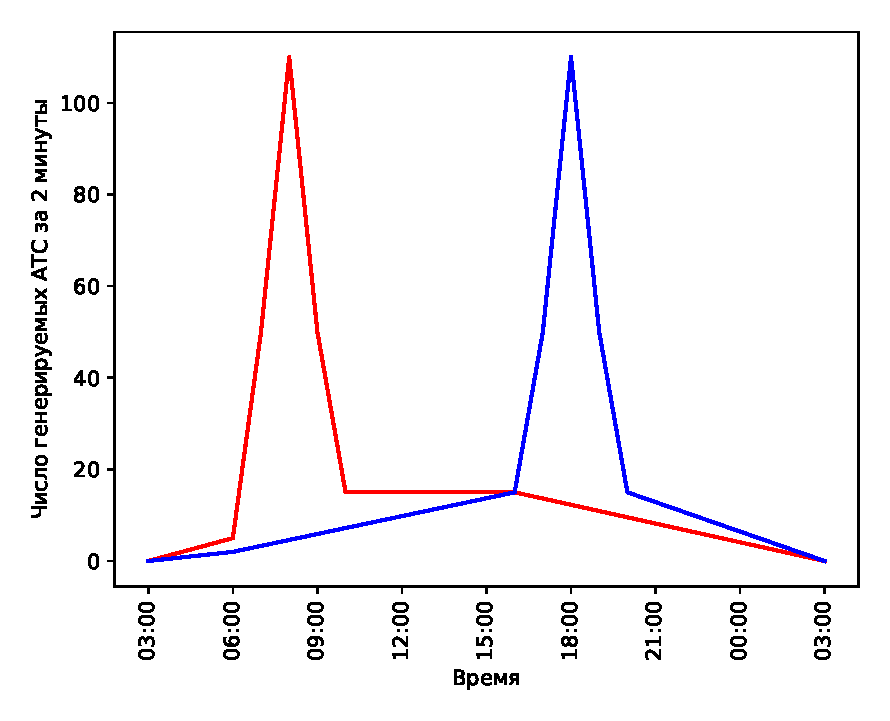
\includegraphics[width=1\linewidth]{MCAR_full_woenters_12_two_types_110_24h_3h_Enters_generators.eps}
        \caption{Графики загрузки двух типов въездов~--- с утренней и вечерней пиковыми загрузками в эксперименте с высокой загрузкой.}
        \label{fig:MCAR_flow_hight_3h}
    \end{minipage}
    \hfill
    \begin{minipage}[b][][b]{0.49\textwidth}
        \centering
        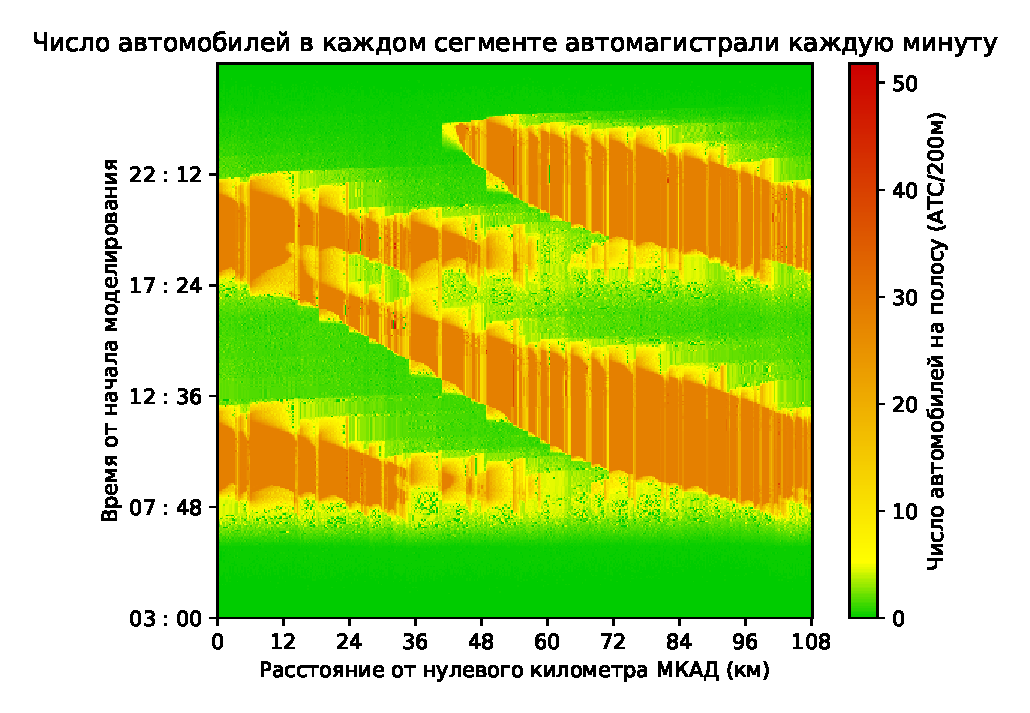
\includegraphics[width=1\linewidth]{MCAR_full_woenters_12_two_types_110_24h_3h.eps}
        \caption{Количество автомобилей на полосу в модели транспортной сети за день в эксперименте с высокой загрузкой.}
        \label{fig:MCAR_heatmap_hight_3h}
    \end{minipage}
\end{figure}

\subsection{Эксперимент без управления въездами}
Результаты моделирования при такой конфигурации въездов представлены на рис.~\ref{fig:MCAR_heatmap_hight_3h}.
Видно, что в данной конфигурации потоков на въездах заторные движения образуются по всей протяженности автомагистрали, объединяясь впоследствии в один большой. В данном эксперименте МКАД практически полностью занят пробкой с утра до вечера.
На рис.~\ref{fig:MCAR_entered_hight_3h} показано число реально въехавших автомобилей и количество проехавших за день по магистрали АТС.
График временных потерь проезда по всей автомагистрали представлен на рис.~\ref{fig:MCAR_timeloss_hight_3h}.

\begin{figure}[ht]
    \begin{minipage}[b][][b]{0.49\textwidth}
        \centering
        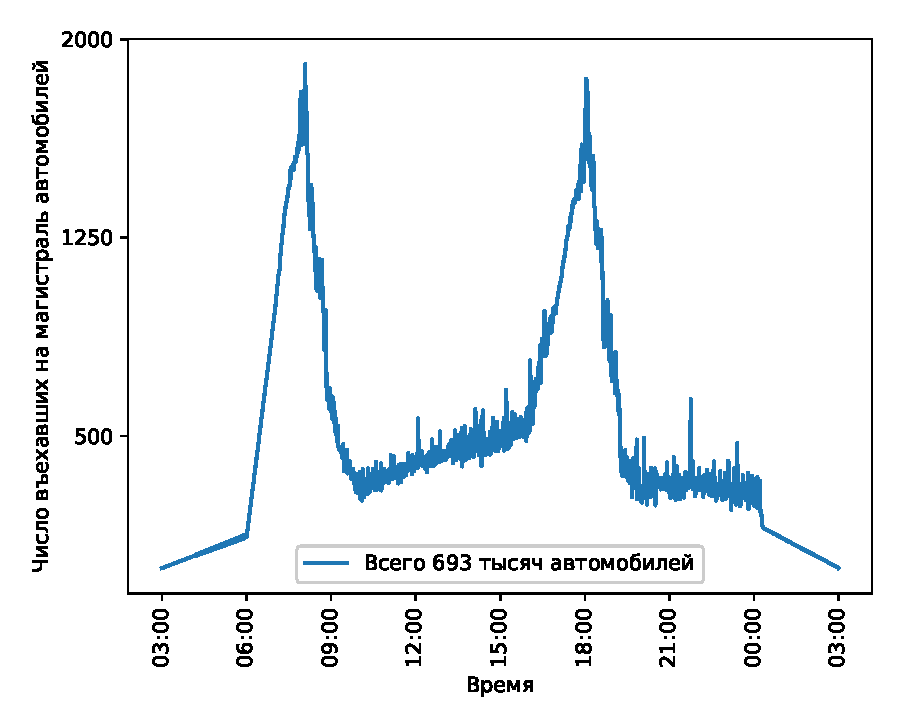
\includegraphics[width=1\linewidth]{MCAR_full_woenters_12_two_types_110_24h_3h_Entered.eps}
        \caption{График суммарно въехавшего на автомагистраль со всех въездов числа автомобилей в эксперименте с высокой загрузкой.}
        \label{fig:MCAR_entered_hight_3h}
    \end{minipage}
    \hfill
    \begin{minipage}[b][][b]{0.49\textwidth}
        \centering
        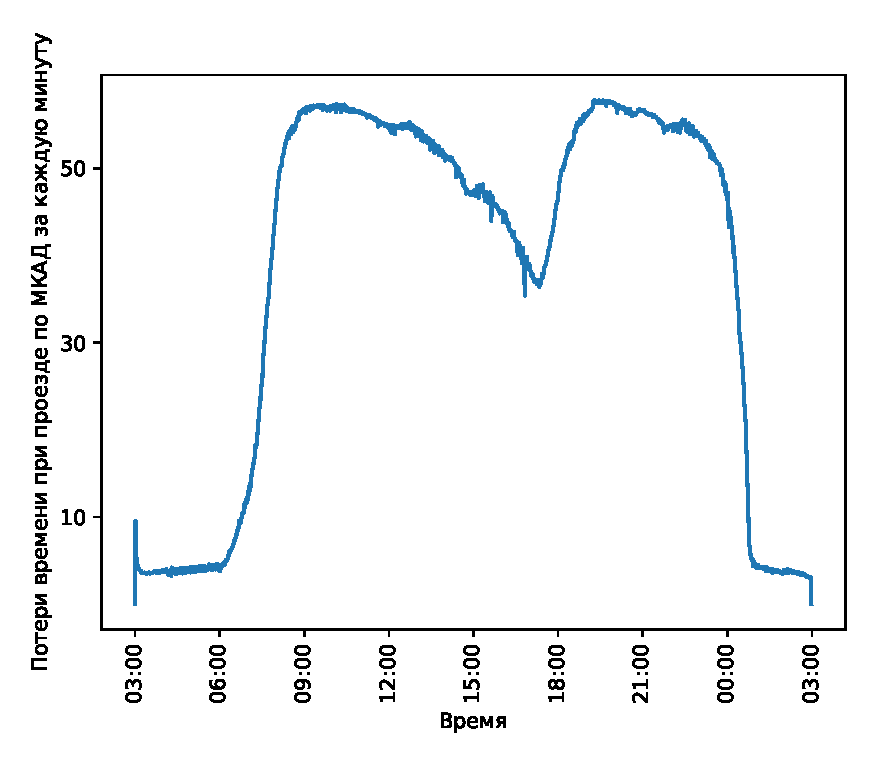
\includegraphics[width=1\linewidth]{MCAR_full_woenters_12_two_types_110_24h_3h_Time_to_pass.eps}
        \caption{Временные потери на проезд по автомагистрали в эксперименте с высокой загрузкой.}
        \label{fig:MCAR_timeloss_hight_3h}
    \end{minipage}
\end{figure}


\subsection{Эксперимент с управлением въездами}
В данном эксперименте с управлением въездами также перекрываем въезды вплоть до 80\% в зависимости от плотности автомобилей на магистрали.
Результаты моделирования, число въехавших автомобилей и график временных потерь при проезде по магистрали изображены на рис.~\ref{fig:MCAR_heatmap_low_3h_handcontrol},~\ref{fig:MCAR_entered_low_3h_handcontrol} и~\ref{fig:MCAR_timeloss_low_3h_handcontrol} соответственно.
\begin{figure}[ht]
    \centerfloat{
        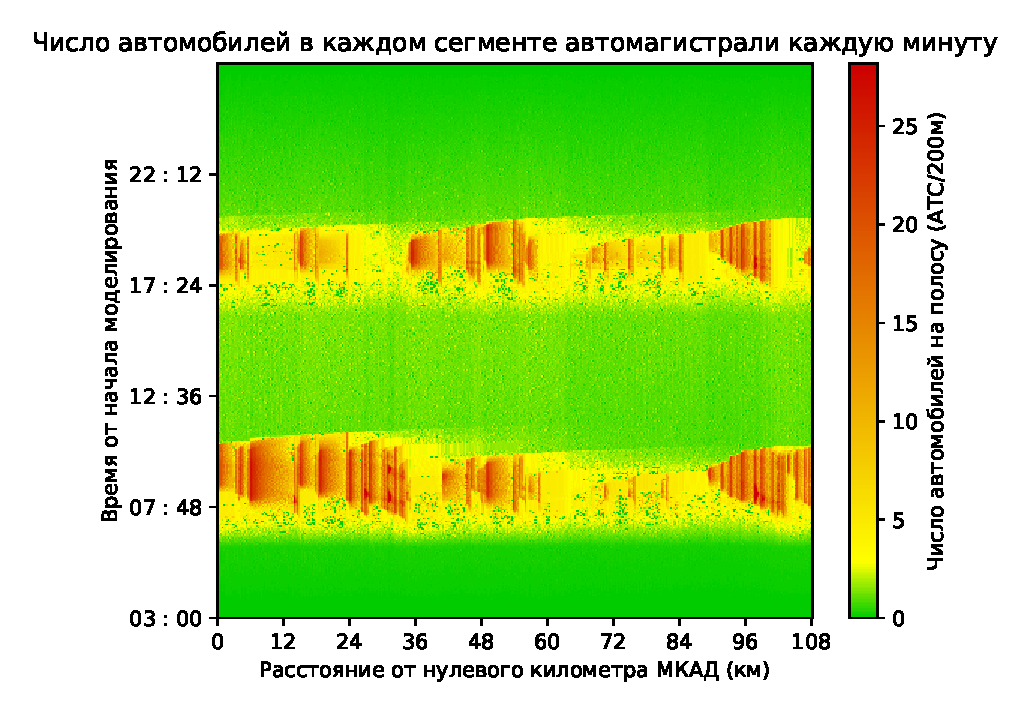
\includegraphics[width=0.8\linewidth]{MCAR_full_woenters_12_two_types_110_24h_3h_handcontrol.eps}
    }
    \caption{Количество автомобилей на полосе в модели транспортной сети за день в эксперименте с высокой загрузкой с управлением въездами.}
    \label{fig:MCAR_heatmap_hight_3h_handcontrol}
\end{figure}

\begin{figure}[ht]
    \begin{minipage}[b][][b]{0.49\textwidth}
        \centering
        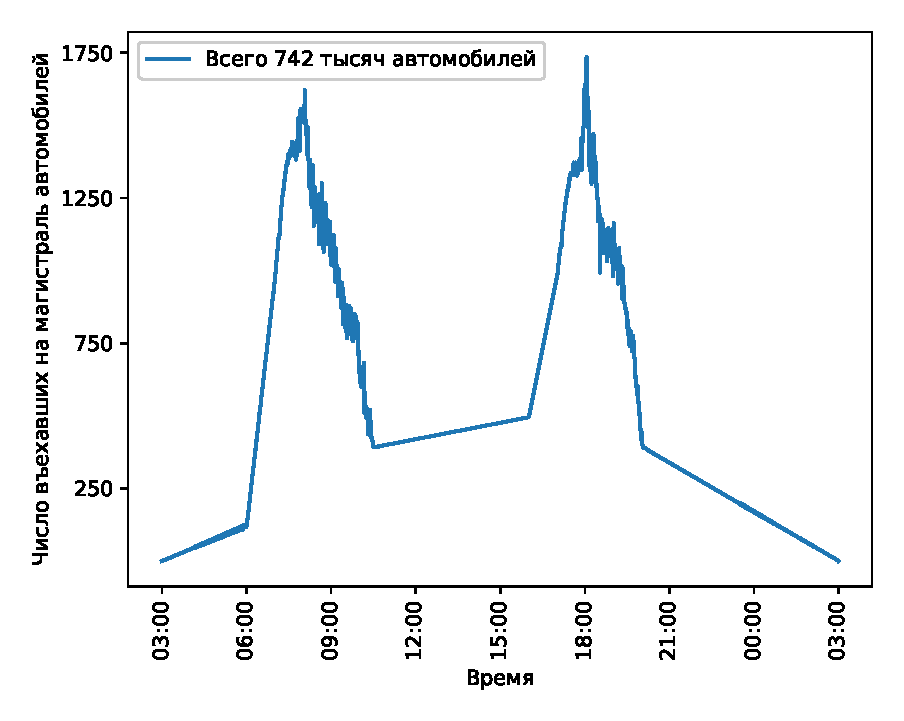
\includegraphics[width=1\linewidth]{MCAR_full_woenters_12_two_types_110_24h_3h_handcontrol_Entered.eps}
        \caption{График суммарно въехавшего на автомагистраль со всех въездов числа автомобилей в эксперименте с высокой загрузкой с управлением въездами.}
        \label{fig:MCAR_entered_hight_3h_handcontrol}
    \end{minipage}
    \hfill
    \begin{minipage}[b][][b]{0.49\textwidth}
        \centering
        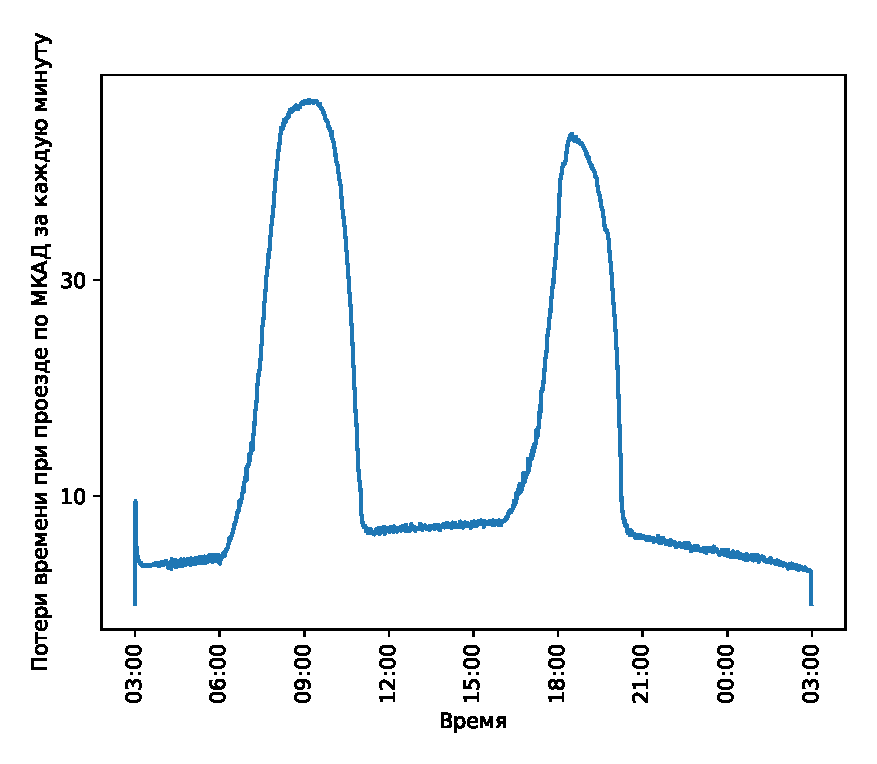
\includegraphics[width=1\linewidth]{MCAR_full_woenters_12_two_types_110_24h_3h_handcontrol_Time_to_pass.eps}
        \caption{Временные потери на проезд по автомагистрали в эксперименте с высокой загрузкой с управлением въездами.}
        \label{fig:MCAR_timeloss_hight_3h_handcontrol}
    \end{minipage}
\end{figure}

На графиках видно уменьшение времени затора на МКАД, а также небольшое увеличение числа проехавших автомобилей.
Хотя число проехавших по МКАД автомобилей увеличилось незначительно, временные потери на проезд по автомагистрали сильно снизились, а временной интервал затрудненного движения уменьшился.
Интегральная разность между графиками на рис.~\ref{fig:MCAR_timeloss_hight_3h}~и~\ref{fig:MCAR_timeloss_hight_3h_handcontrol} составляет чуть более $18$ минут.

\section{Эксперименты с высокой загрузкой с длинными въездами}
В данной группе экспериментов функции входного потока соответствуют потоку в предыдущем эксперименте и изображены на рис.~\ref{fig:MCAR_flow_hight_3h}.
В данном случае у нас есть два типа въездов на автомагистраль~--- с утренней и вечерней пиковыми загрузками в течение трех часов.
Въезды на автомагистраль~- все протяженностью в $6$ километров в отличие от уже проведенных экспериментов, в которых их длина бралась $2$ километра.

В данном разделе приведем все результирующие графики парами.
Результаты моделирования представлены на рис.~\ref{fig:MCAR_heatmap_hight_3h_6km}.
Число реально въехавших автомобилей и количество проехавших за день по магистрали АТС изображены на рис.~\ref{fig:MCAR_entered_hight_3h_6km}.
График временных потерь проезда по всей автомагистрали представлен на рис.~\ref{fig:MCAR_timeloss_hight_3h_6km}.
График временных потерь въезда на автомагистрали относительно пустой транспортной сети показан на рис.~\ref{fig:MCAR_timeloss_enter_hight_3h_6km}.

В эксперименте видно, что из-за большого числа автомобилей, ожидающих въезда на МКАД без управления въездами, автомагистраль полностью забивается и не успевает освободиться до конца моделирования.
Поскольку динамическое управление въездами не позволяет пробке поддерживаться за счет ограничения входного потока на магистраль, наблюдается значительное улучшение состояния магистрали и сильная локализация затора во времени.

Интегральная разность между графиками на рис.~\ref{fig:MCAR_timeloss_enter_hight_3h_6km} составляет чуть более $26$ минут.
Однако имеет смысл не учитывать сугубо экстремальную вечернюю ситуацию с практически полной остановкой автомагистрали. В этом случае при расчете интеграла до 15:00 задержка ожидания проезда по МКАД составит около $7$ минут за половину суток.

\begin{figure}[ht]
    \begin{minipage}[b][][b]{0.49\textwidth}
        \centering
        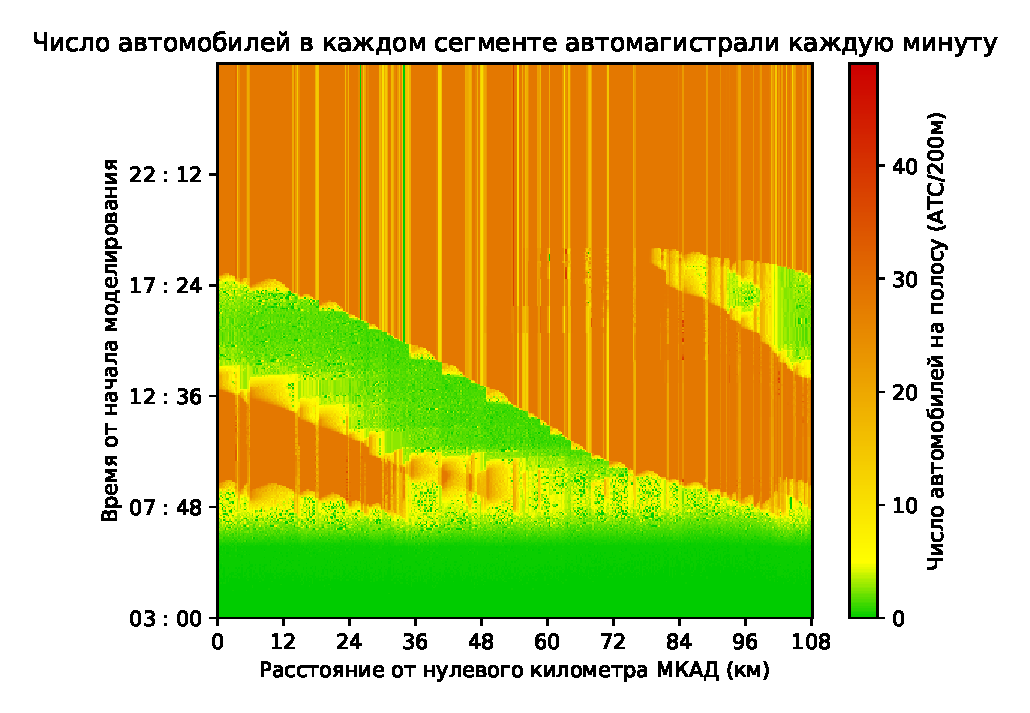
\includegraphics[width=1\linewidth]{MCAR_full_woenters_12_two_types_110_24h_3h_6km.eps} \\ а) Без управления въездами
    \end{minipage}
    \hfill
    \begin{minipage}[b][][b]{0.49\textwidth}
        \centering
        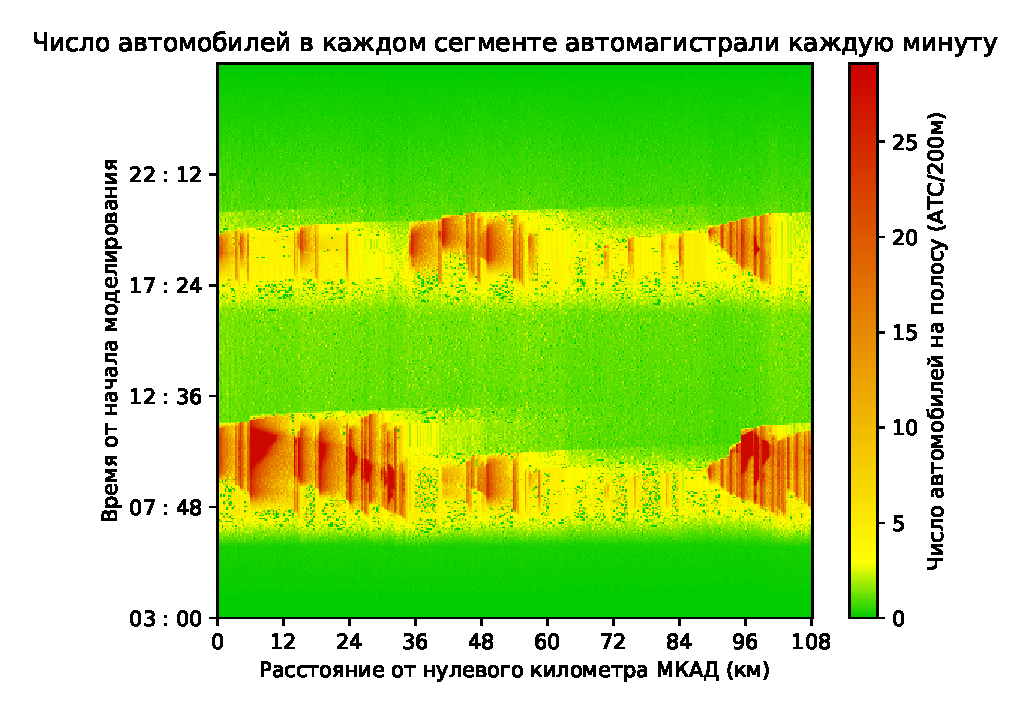
\includegraphics[width=1\linewidth]{MCAR_full_woenters_12_two_types_110_24h_3h_6km_handcontrol.eps} \\ б) С управлением въездами
    \end{minipage}

    \caption{Количество автомобилей на полосу в модели транспортной сети за день в эксперименте с высокой загрузкой.}
    \label{fig:MCAR_heatmap_hight_3h_6km}
\end{figure}

\begin{figure}[ht]
    \begin{minipage}[b][][b]{.49\textwidth}
        \centering
        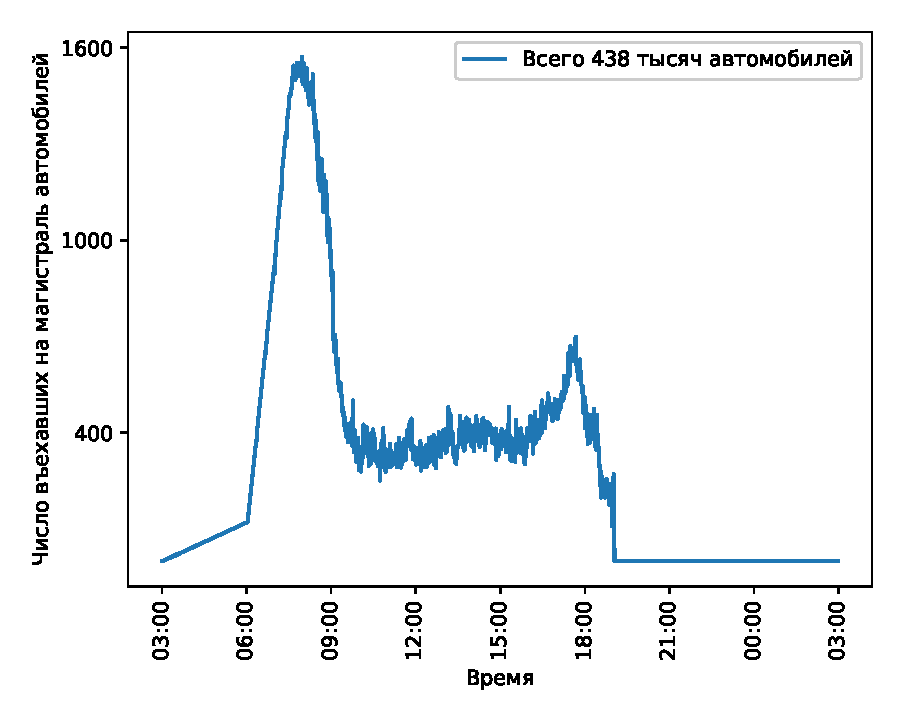
\includegraphics[width=1\linewidth]{MCAR_full_woenters_12_two_types_110_24h_3h_6km_Entered.eps} \\ а) Без управления въездами
    \end{minipage}
    \hfill
    \begin{minipage}[b][][b]{.49\textwidth}
        \centering
        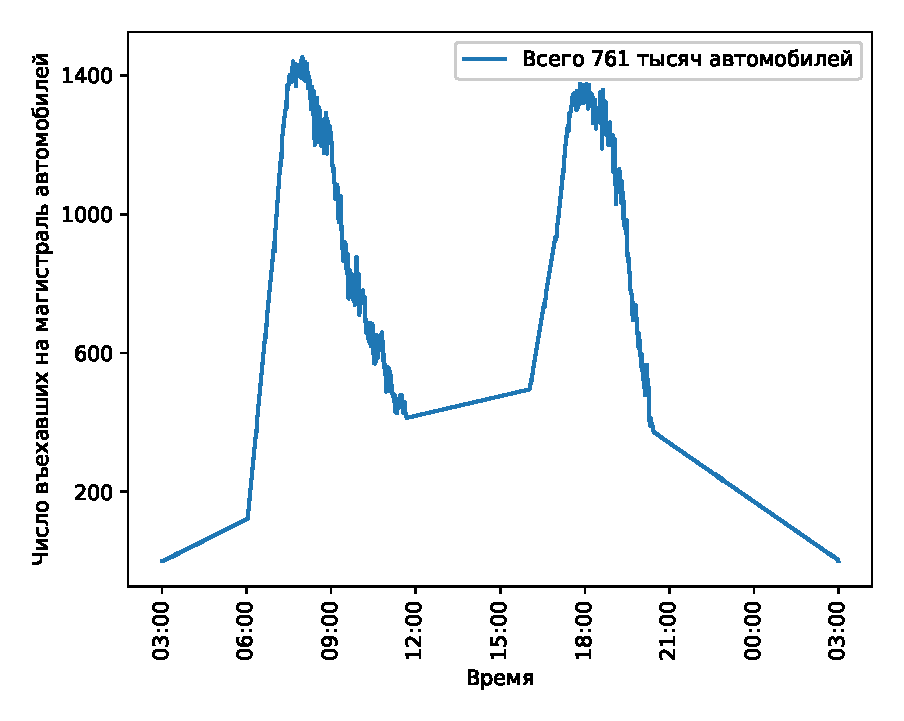
\includegraphics[width=1\linewidth]{MCAR_full_woenters_12_two_types_110_24h_3h_6km_handcontrol_Entered.eps} \\ б) С управлением въездами
    \end{minipage}

    \caption{Графики суммарно въехавшего на автомагистраль со всех въездов числа автомобилей в эксперименте с высокой загрузкой.}
    \label{fig:MCAR_entered_hight_3h_6km}
\end{figure}


\begin{figure}[ht]
    \begin{minipage}[b][][b]{.49\textwidth}
        \centering
        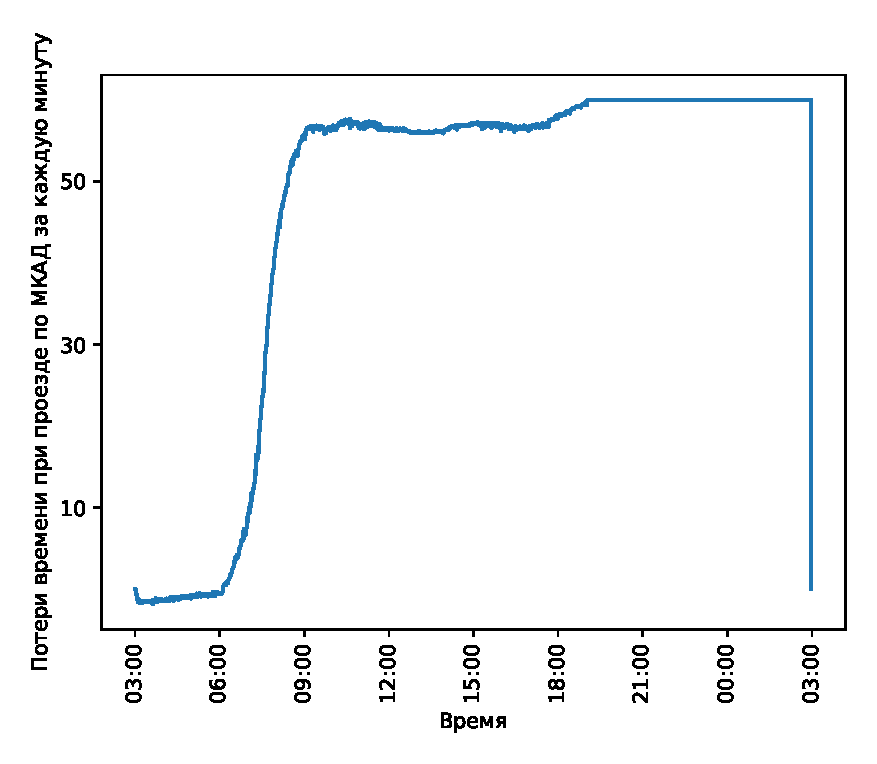
\includegraphics[width=1\linewidth]{MCAR_full_woenters_12_two_types_110_24h_3h_6km_Time_to_pass.eps} \\ а) Без управления въездами
    \end{minipage}
    \hfill
    \begin{minipage}[b][][b]{.49\textwidth}
        \centering
        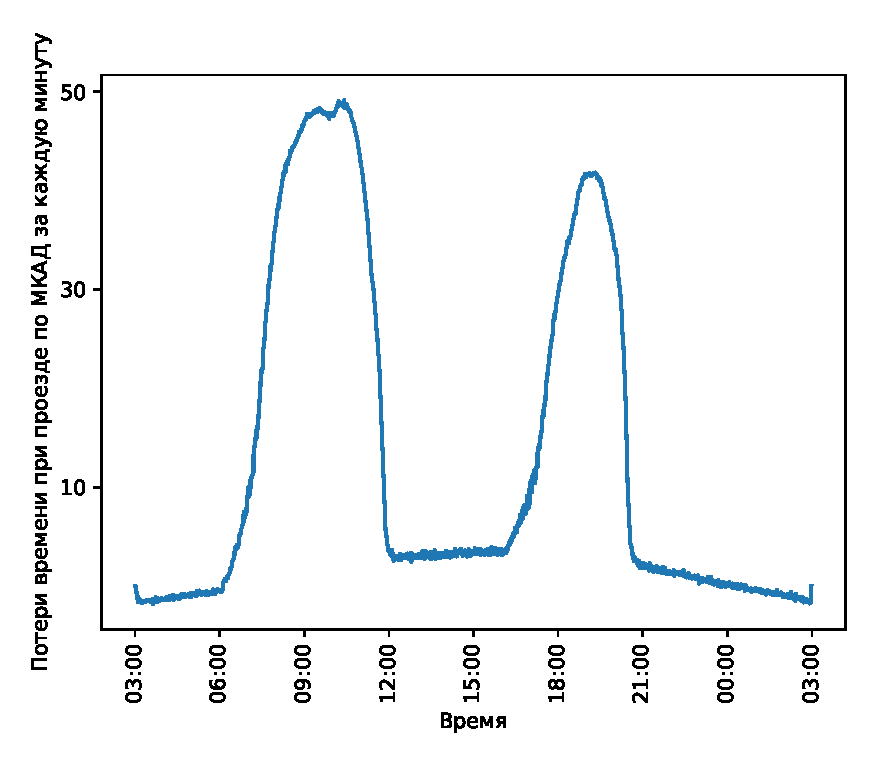
\includegraphics[width=1\linewidth]{MCAR_full_woenters_12_two_types_110_24h_3h_6km_handcontrol_Time_to_pass.eps} \\ б) С управлением въездами
    \end{minipage}

    \caption{Временные потери на проезд по автомагистрали в эксперименте с высокой загрузкой.}
    \label{fig:MCAR_timeloss_hight_3h_6km}
\end{figure}

\begin{figure}[ht]
    \begin{minipage}[b][][b]{.49\textwidth}
        \centering
        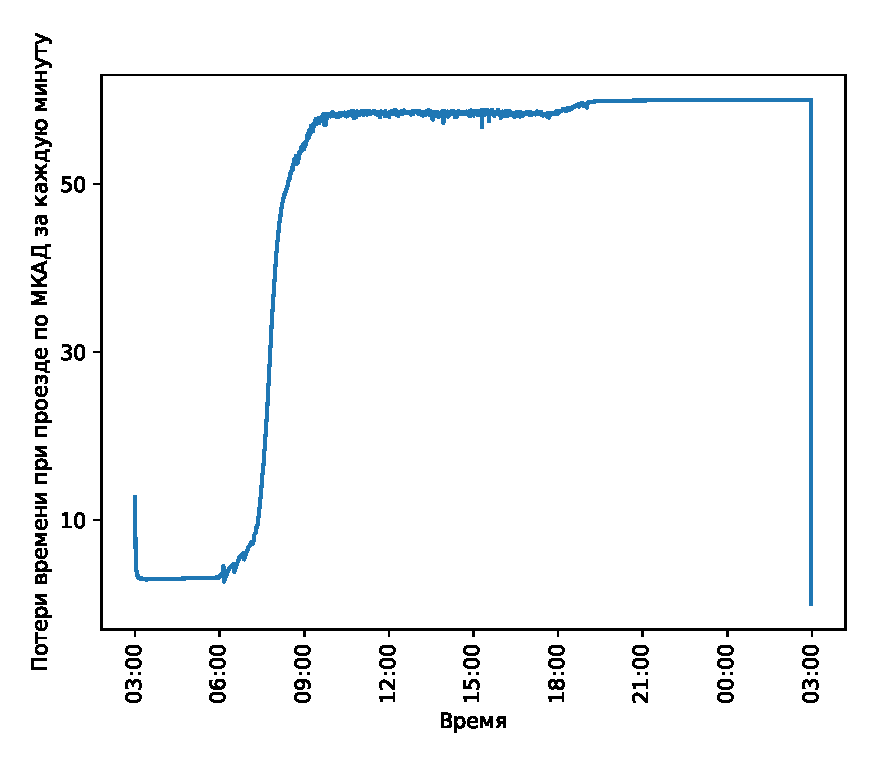
\includegraphics[width=1\linewidth]{MCAR_full_woenters_12_two_types_110_24h_3h_6km_Time_to_enter.eps}  \\ а) Без управления въездами
    \end{minipage}
    \hfill
    \begin{minipage}[b][][b]{.49\textwidth}
        \centering
        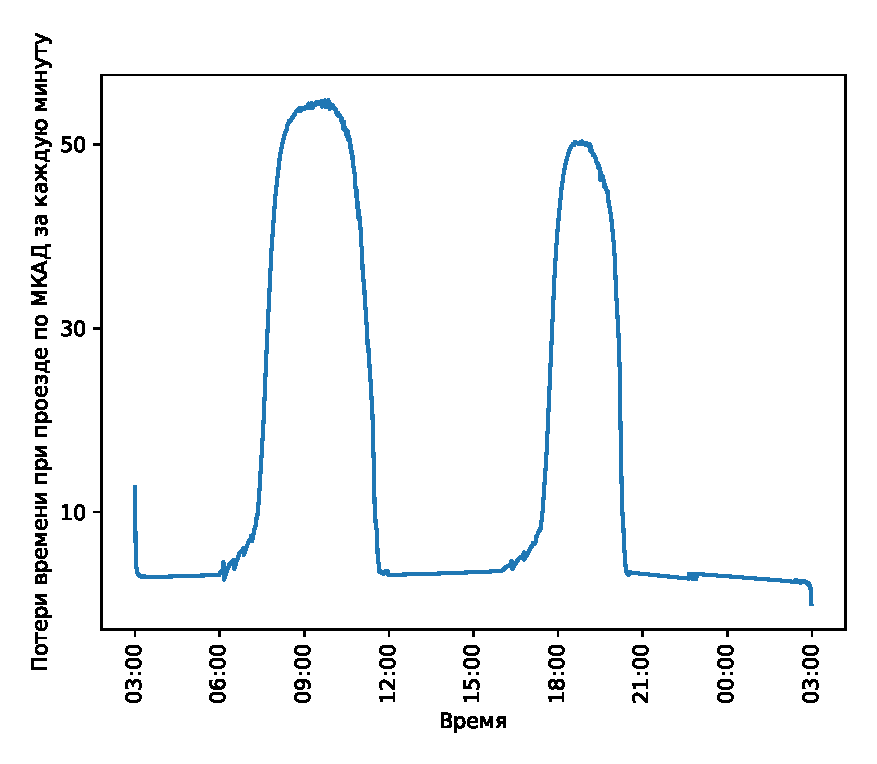
\includegraphics[width=1\linewidth]{MCAR_full_woenters_12_two_types_110_24h_3h_6km_handcontrol_Time_to_enter.eps}  \\ b) С управлением въездами
    \end{minipage}

    \caption{Временные потери на въезд на автомагистраль в эксперименте с высокой загрузкой.}
    \label{fig:MCAR_timeloss_enter_hight_3h_6km}
\end{figure}



\chapter{Моделирование МКАД с вычислением всех фундаментальных диаграмм}\label{sec:ch6}
В данном разделе описываются эксперименты, аналогичные проведенным в разделе~\ref{sec::experiments} однако теперь для каждого сегмента МКАД была рассчитана соответствующая ему фундаментальная диаграмма на основе данных с дорожных датчиков
расположенных над этим сегментом либо рядом с ним.
Проводятся следующие группы экспериментов:
\begin{enumerate}
  \item Эксперименты со средней, но продолжительной, пиковой загрузкой на въезды с проверкой эффекта от динамического ограничения входного потока в зависимости от состояния автомагистрали.
  \item Эксперименты с высокой, но непродолжительной, пиковой загрузкой въездов (что более соответствует данным от ЦОДД) с проверкой эффекта от динамического ограничения входного потока в зависимости от состояния автомагистрали.
\end{enumerate}

В данном разделе принимаются все те же предположения что и в разделе~\ref{sec::experiments}, а конкретно~--- доля съезжающих автомобилей равна \(12\%\), а управление въездами происходит по аналогичному алгоритму:
\begin{itemize}
  \item Для каждого сегмента автомагистрали по направлению движения АТС после рассматриваемого въезда посчитаем плотность автомобилей \(\rho\) на ней.
  \item В зависимости от величины \(\rho_{\text{opt}} - \rho$, где $\rho_{\text{opt}}\)~--- плотность, при которой достигается максимальный поток на рассматриваемом сегменте автомагистрали, входной поток ограничивается на \(l<l_{\text{max}}\) процентов.
  \item Ограничения для каждого из сегментов складываются и получается результирующее понижение входного потока АТС.
\end{itemize}

\section{Эксперименты со средней загрузкой}
\label{sec:ch6/average_FD}
В данной группе экспериментов въезды считаются однополосными и функции входного потока изображены на рис.~\ref{fig:MCAR_flow_low_3h}.
В данном случае есть два типа въездов на автомагистраль~--- с утренней и вечерней пиковыми загрузками в течение трех часов.
\begin{figure}[ht]
    \centerfloat{
        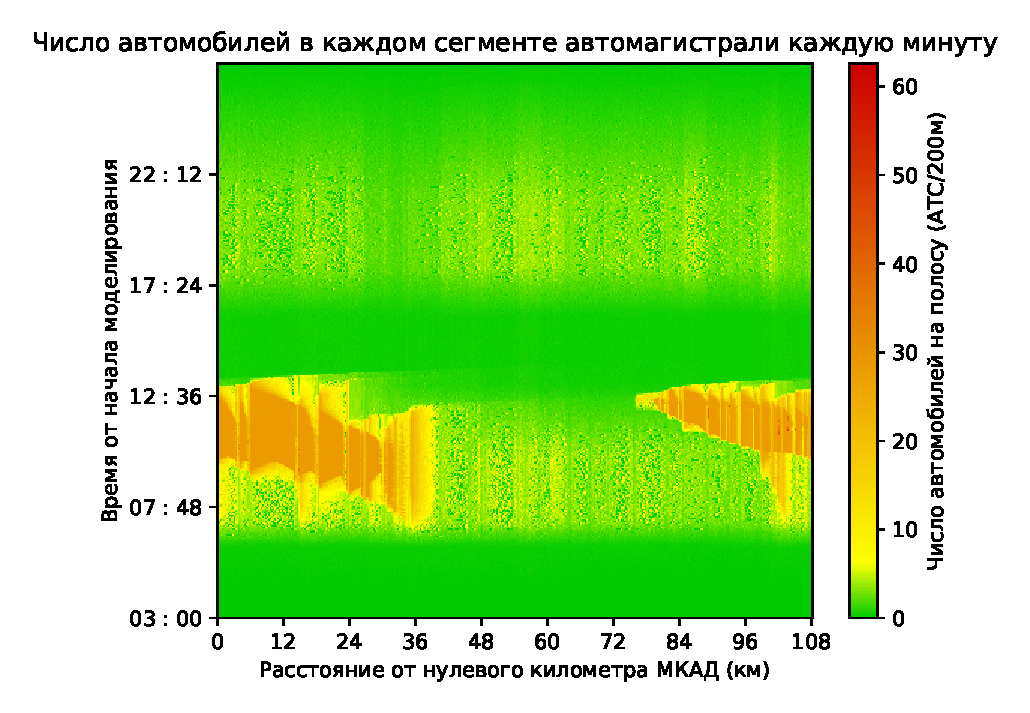
\includegraphics[width=0.8\linewidth]{MCAR_full_woenters_12_two_types_60_24h_3hmax_fullFD.eps}
    }
    \caption{Количество автомобилей на полосе в модели транспортной сети за день в эксперименте со средней загрузкой с расчетом всех фундаментальных диаграмм.}
    \label{fig:MCAR_heatmap_low_3h_FD}
\end{figure}

\subsection{Эксперимент без управления въездами}
Результаты моделирования автомагистрали при такой конфигурации въездов представлены на рис.~\ref{fig:MCAR_heatmap_low_3h_FD}.
Число реально въехавших автомобилей и количество проехавших за день по транспортной сети АТС изображены на рис.~\ref{fig:MCAR_entered_low_3h_FD}.
График временных потерь~- на рис.~\ref{fig:MCAR_timeloss_low_3h_FD}.

Видно, что при такой конфигурации входных потоков заторы возникают всего в нескольких местах и потом со временем распространяются по автомагистрали.
Так как пробки успевают исчезнуть к вечеру, то МКАД не останавливается полностью, хотя при меньшей доли съезжающих автомобилей это произойдет.
В сравнении с аналогичным экспериментом из предыдущего раздела пробка исчезает быстрее при спаде входного потока АТС.
\begin{figure}[ht]
    \begin{minipage}[b][][b]{0.49\textwidth}
        \centering
        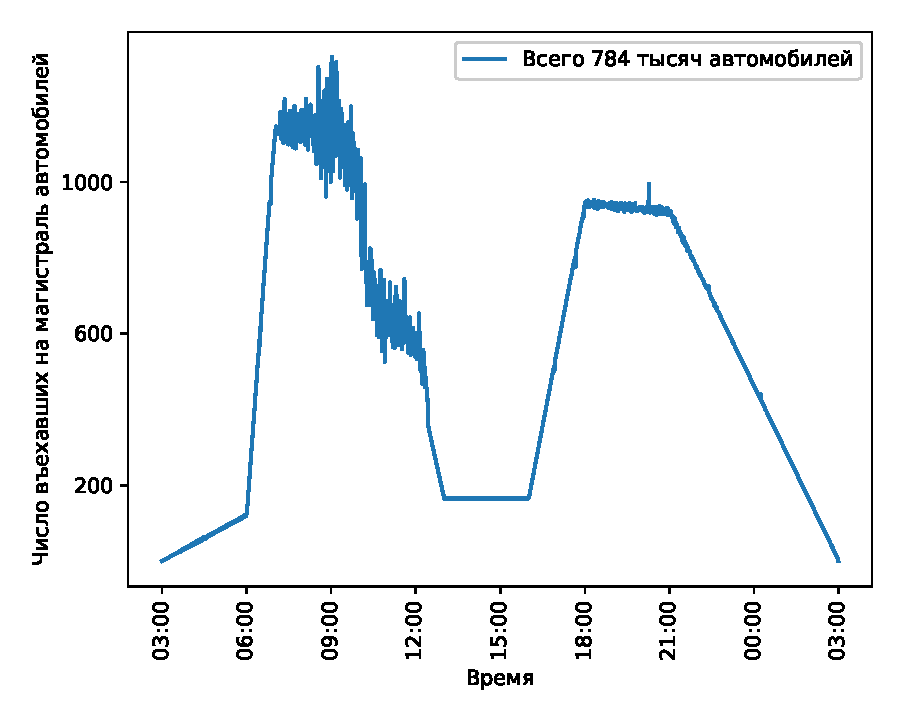
\includegraphics[width=1\linewidth]{MCAR_full_woenters_12_two_types_60_24h_3hmax_fullFD_Entered.eps}
        \caption{График суммарно въехавшего на автомагистраль со всех въездов числа автомобилей в эксперименте со средней загрузкой с расчетом всех фундаментальных диаграмм.}
        \label{fig:MCAR_entered_low_3h_FD}
    \end{minipage}
    \hfill
    \begin{minipage}[b][][b]{0.49\textwidth}
        \centering
        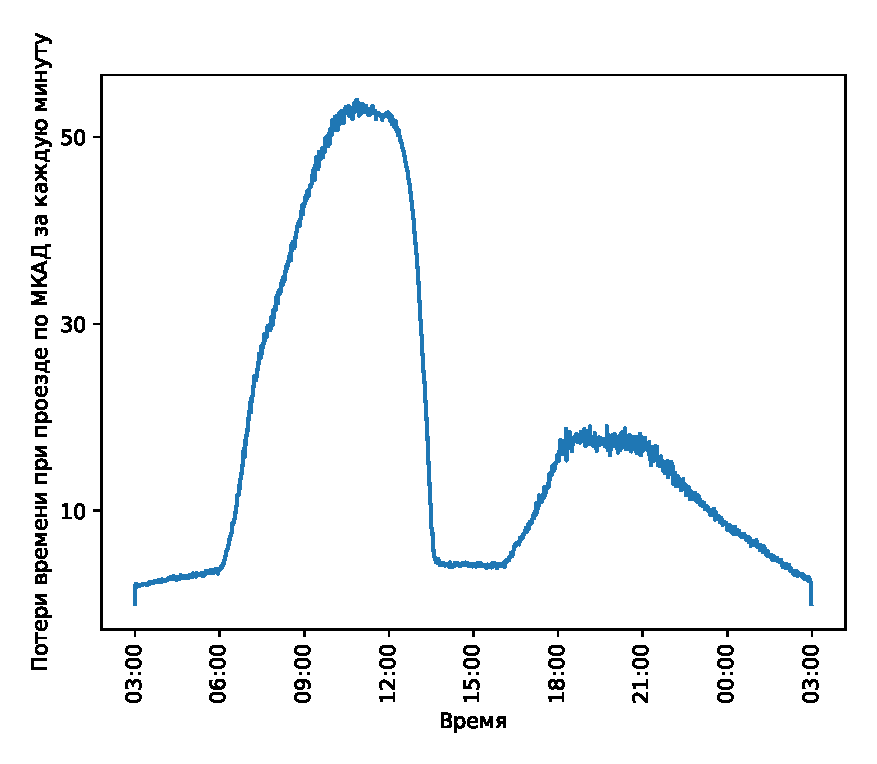
\includegraphics[width=1\linewidth]{MCAR_full_woenters_12_two_types_60_24h_3hmax_fullFD_Time_to_pass.eps}
        \caption{Временные потери на проезд по автомагистрали в эксперименте со средней загрузкой с расчетом всех фундаментальных диаграмм.}
        \label{fig:MCAR_timeloss_low_3h_FD}
    \end{minipage}
\end{figure}


\subsection{Эксперимент с управлением въездами}
Аналогично предыдущему разделу промоделируем ситуацию светофорного управления въездами с возможностью перекрывать вплоть до 80\% входного потока.
Результаты моделирования при такой конфигурации въездов представлены на рис.~\ref{fig:MCAR_heatmap_low_3h_handcontrol_FD}.
Число реально въехавших автомобилей и количество проехавших за день по транспортной сети АТС изображены на рис.~\ref{fig:MCAR_entered_low_3h_handcontrol_FD}.
График временных потерь проезда по всей автомагистрали представлен на рис.~\ref{fig:MCAR_timeloss_low_3h_handcontrol_FD}.
\begin{figure}[ht]
    \centerfloat{
        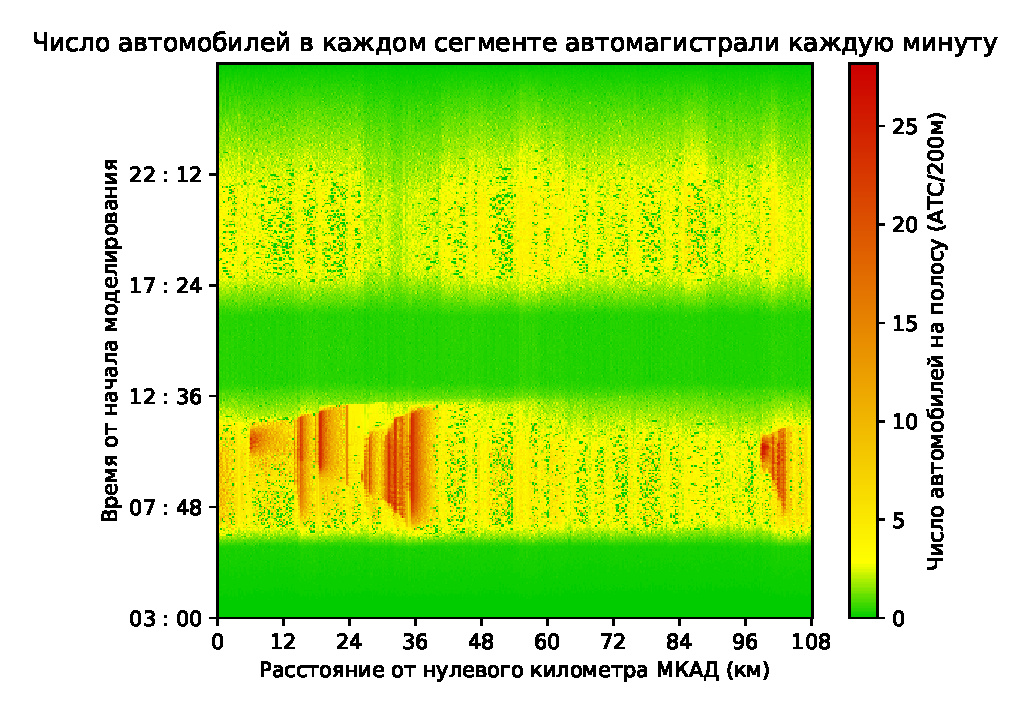
\includegraphics[width=0.8\linewidth]{MCAR_full_woenters_12_two_types_60_24h_3hmax_fullFD_handcontrol.eps}
    }
    \caption{Количество автомобилей на полосе в модели транспортной сети за день в эксперименте со средней загрузкой с управлением въездами с расчетом всех фундаментальных диаграмм.}
    \label{fig:MCAR_heatmap_low_3h_handcontrol_FD}
\end{figure}

\begin{figure}[ht]
    \begin{minipage}[b][][b]{0.49\textwidth}
        \centering
        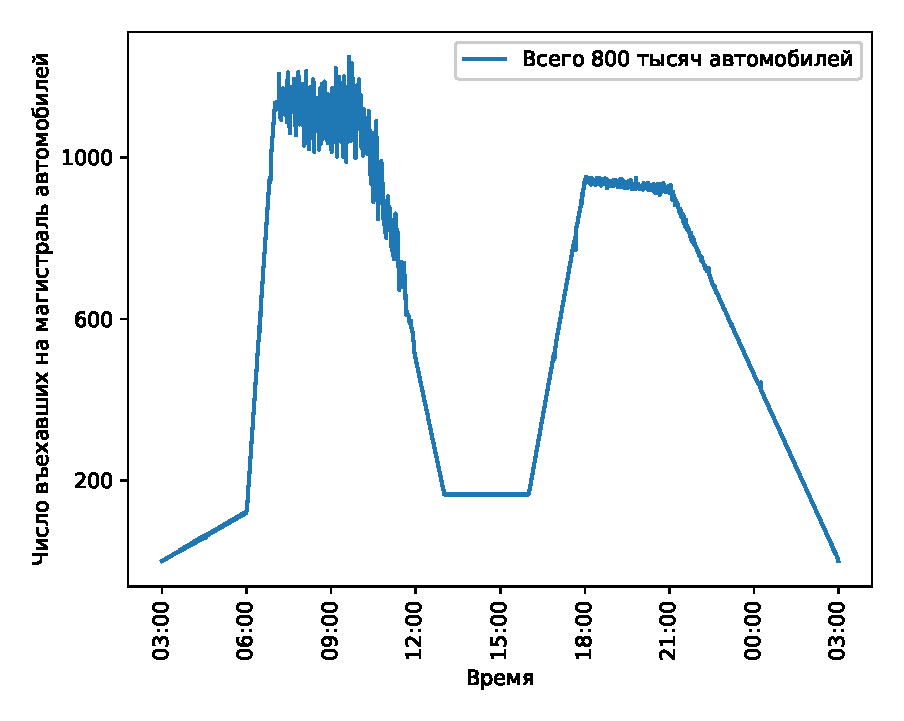
\includegraphics[width=1\linewidth]{MCAR_full_woenters_12_two_types_60_24h_3hmax_fullFD_handcontrol_Entered.eps}
        \caption{График суммарно въехавшего на автомагистраль со всех въездов числа автомобилей в эксперименте со средней загрузкой с управлением въездами с расчетом всех фундаментальных диаграмм.}
        \label{fig:MCAR_entered_low_3h_handcontrol_FD}
    \end{minipage}
    \hfill
    \begin{minipage}[b][][b]{0.49\textwidth}
        \centering
        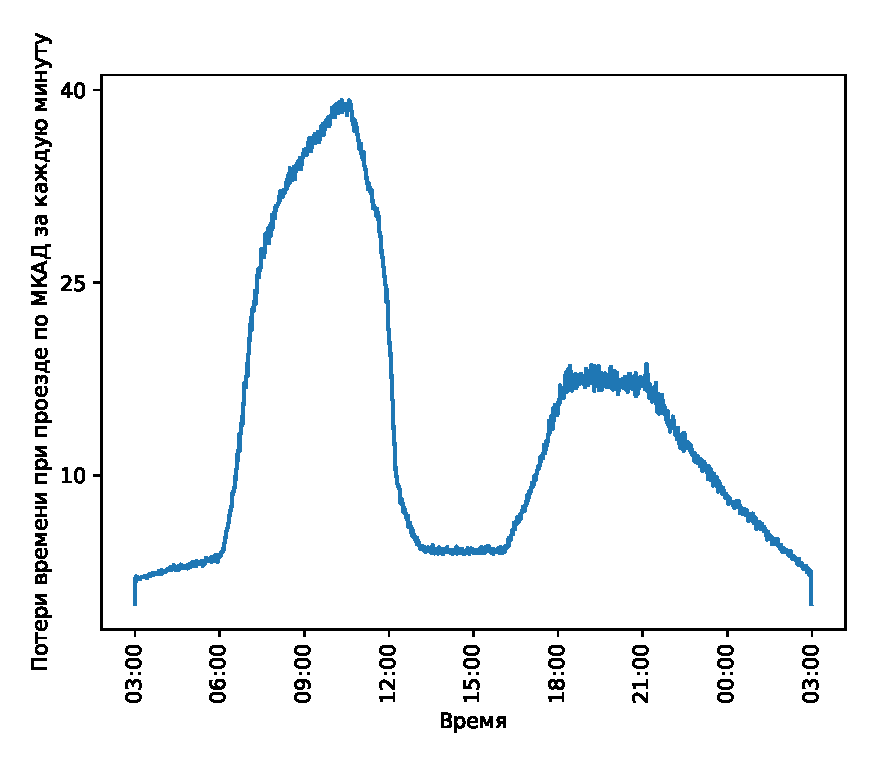
\includegraphics[width=1\linewidth]{MCAR_full_woenters_12_two_types_60_24h_3hmax_fullFD_handcontrol_Time_to_pass.eps}
        \caption{Временные потери на проезд по автомагистрали в эксперименте со средней загрузкой с управлением въездами с расчетом всех фундаментальных диаграмм.}
        \label{fig:MCAR_timeloss_low_3h_handcontrol_FD}
    \end{minipage}
\end{figure}

На графиках видно уменьшение времени затора на МКАД, а также небольшое увеличение числа проехавших автомобилей.
Однако временные потери на проезд по автомагистрали значительно снизились.
Интегральная разность между графиками временных потерь на рис.~\ref{fig:MCAR_timeloss_low_3h_FD}~и~\ref{fig:MCAR_timeloss_low_3h_handcontrol_FD} составляет около $1$ минуты.
Видно, что при низкой загрузке и более аккуратном моделировании с учетом всех фундаментальных диаграмм эффективность управления въездами достаточно сильно упала.


\section{Эксперименты с высокой загрузкой}
\label{sec:ch6/hight_FD}
В данной группе экспериментов въезды считаются двухполосными и функции входного потока изображены на рис.~\ref{fig:MCAR_flow_hight_3h}.
В данном случае есть два типа въездов на автомагистраль~--- с утренней и вечерней пиковыми загрузками в течение трех часов.

\begin{figure}[ht]
    \centerfloat{
        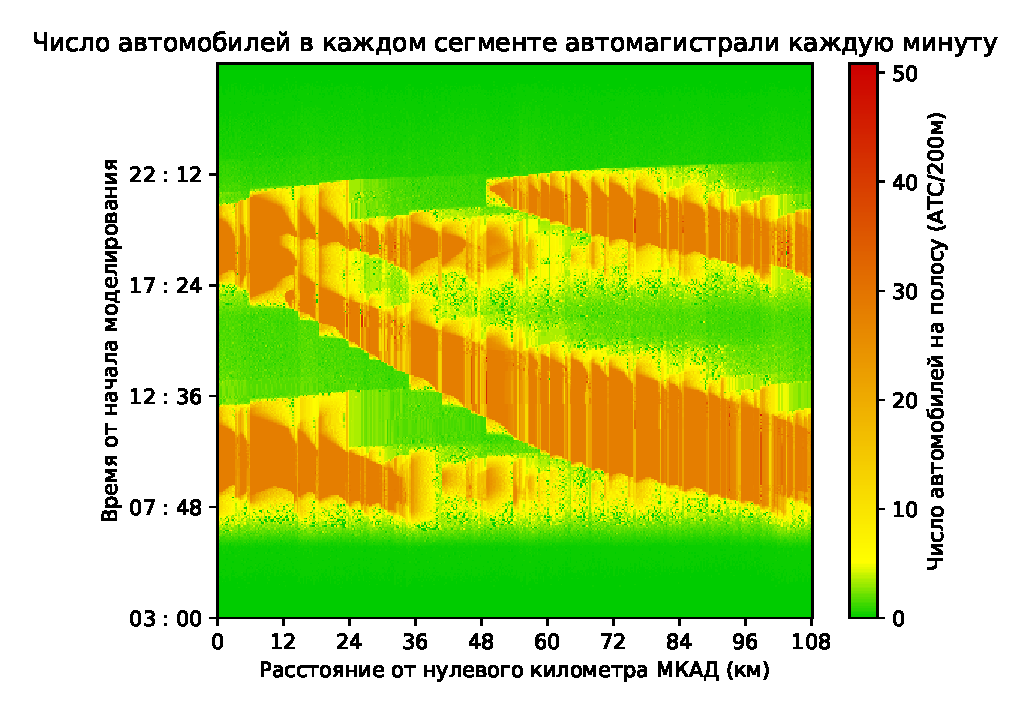
\includegraphics[width=0.8\linewidth]{MCAR_full_woenters_12_two_types_110_24h_3h_fullFD.eps}
    }
    \caption{Количество автомобилей на полосу в модели транспортной сети за день в эксперименте с высокой загрузкой с расчетом всех фундаментальных диаграмм.}
    \label{fig:MCAR_heatmap_hight_3h_FD}
\end{figure}


\subsection{Эксперимент без управления въездами}
Результаты моделирования при такой конфигурации въездов представлены на рис.~\ref{fig:MCAR_heatmap_hight_3h_FD}.
Видно, что в данной конфигурации потоков на въездах заторные движения образуются по всей протяженности автомагистрали, объединяясь впоследствии в один большой.
В данном эксперименте, аналогично эксперименту из предыдущего раздела, МКАД практически полностью занят пробкой с утра до вечера.
На рис.~\ref{fig:MCAR_entered_hight_3h} показано число реально въехавших автомобилей и количество проехавших за день по магистрали АТС.
График временных потерь проезда по всей автомагистрали представлен на рис.~\ref{fig:MCAR_timeloss_hight_3h_FD}.

\begin{figure}[ht]
    \begin{minipage}[b][][b]{0.49\textwidth}
        \centering
        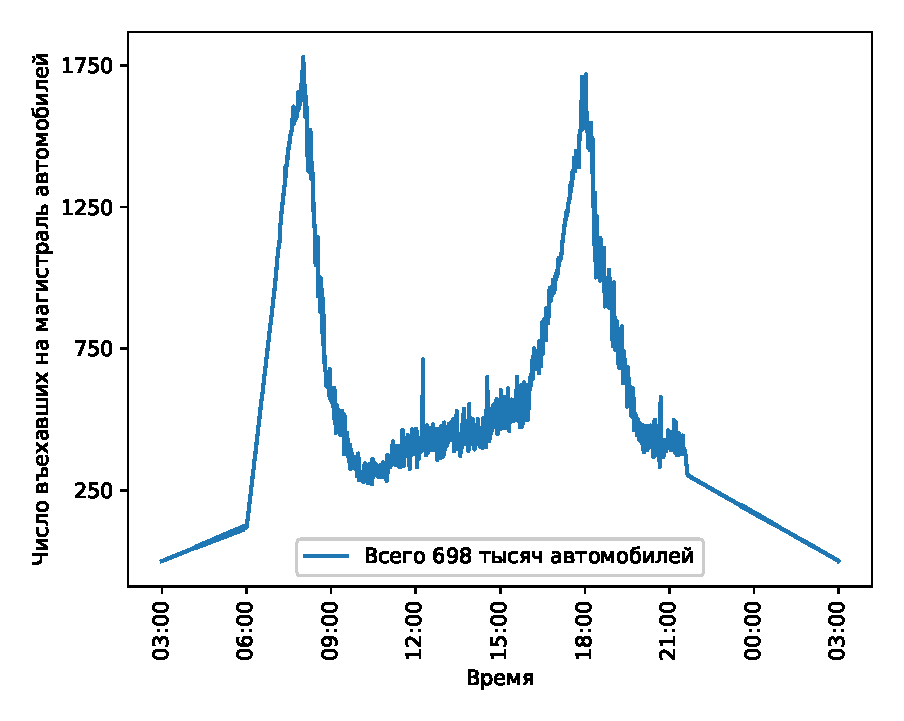
\includegraphics[width=1\linewidth]{MCAR_full_woenters_12_two_types_110_24h_3h_fullFD_Entered.eps}
        \caption{График суммарно въехавшего на автомагистраль со всех въездов числа автомобилей в эксперименте с высокой загрузкой с расчетом всех фундаментальных диаграмм.}
        \label{fig:MCAR_entered_hight_3h_FD}
    \end{minipage}
    \hfill
    \begin{minipage}[b][][b]{0.49\textwidth}
        \centering
        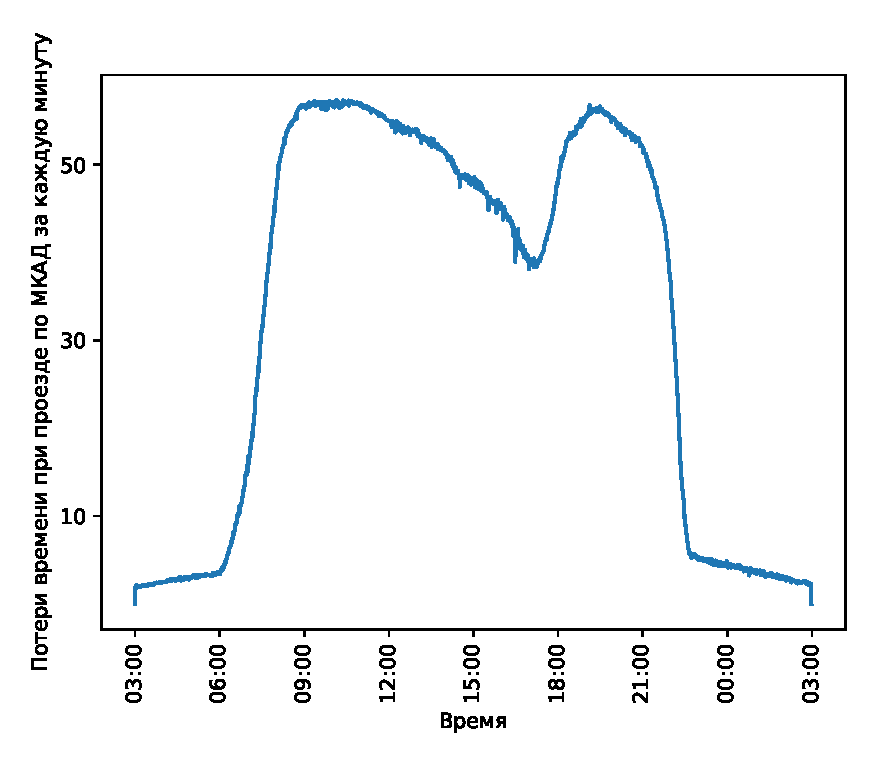
\includegraphics[width=1\linewidth]{MCAR_full_woenters_12_two_types_110_24h_3h_fullFD_Time_to_pass.eps}
        \caption{Временные потери на проезд по автомагистрали в эксперименте с высокой загрузкой с расчетом всех фундаментальных диаграмм.}
        \label{fig:MCAR_timeloss_hight_3h_FD}
    \end{minipage}
\end{figure}


\subsection{Эксперимент с управлением въездами}
В данном эксперименте с управлением въездами также перекрываем въезды вплоть до 80\% в зависимости от плотности автомобилей на магистрали.
Результаты моделирования, число въехавших автомобилей и график временных потерь при проезде по магистрали изображены на рис.~\ref{fig:MCAR_heatmap_low_3h_handcontrol},~\ref{fig:MCAR_entered_low_3h_handcontrol} и~\ref{fig:MCAR_timeloss_low_3h_handcontrol} соответственно.
\begin{figure}[ht]
    \centerfloat{
        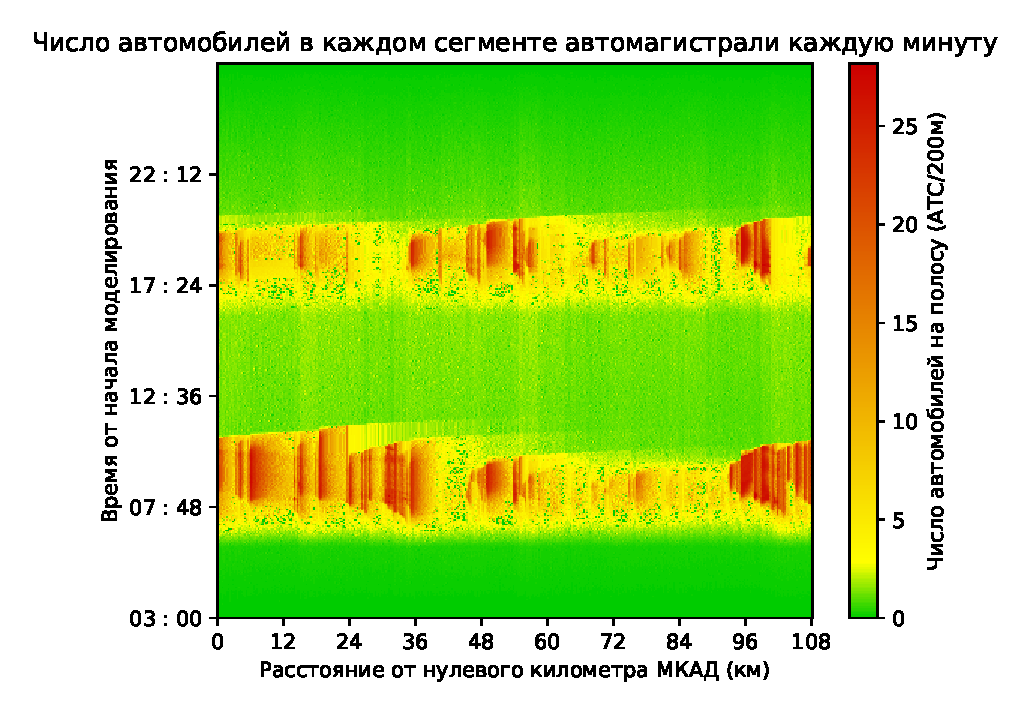
\includegraphics[width=0.8\linewidth]{MCAR_full_woenters_12_two_types_110_24h_3h_fullFD_handcontrol.eps}
    }
    \caption{Количество автомобилей на полосе в модели транспортной сети за день в эксперименте с высокой загрузкой с управлением въездами с расчетом всех фундаментальных диаграмм.}
    \label{fig:MCAR_heatmap_hight_3h_handcontrol_FD}
\end{figure}

\begin{figure}[ht]
    \begin{minipage}[b][][b]{0.49\textwidth}
        \centering
        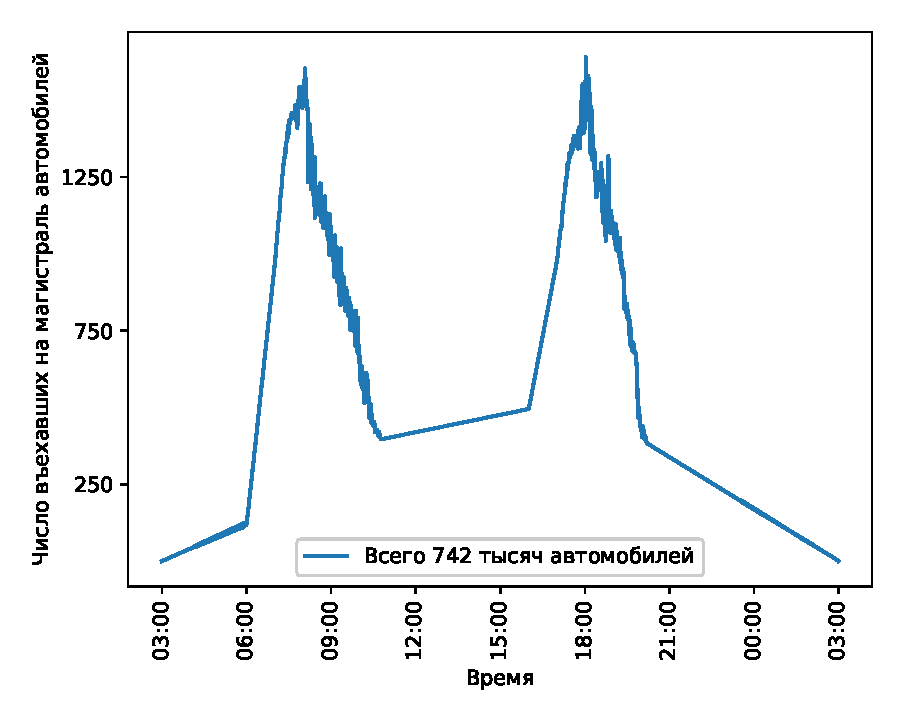
\includegraphics[width=1\linewidth]{MCAR_full_woenters_12_two_types_110_24h_3h_fullFD_handcontrol_Entered.eps}
        \caption{График суммарно въехавшего на автомагистраль со всех въездов числа автомобилей в эксперименте с высокой загрузкой с управлением въездами с расчетом всех фундаментальных диаграмм.}
        \label{fig:MCAR_entered_hight_3h_handcontrol_FD}
    \end{minipage}
    \hfill
    \begin{minipage}[b][][b]{0.49\textwidth}
        \centering
        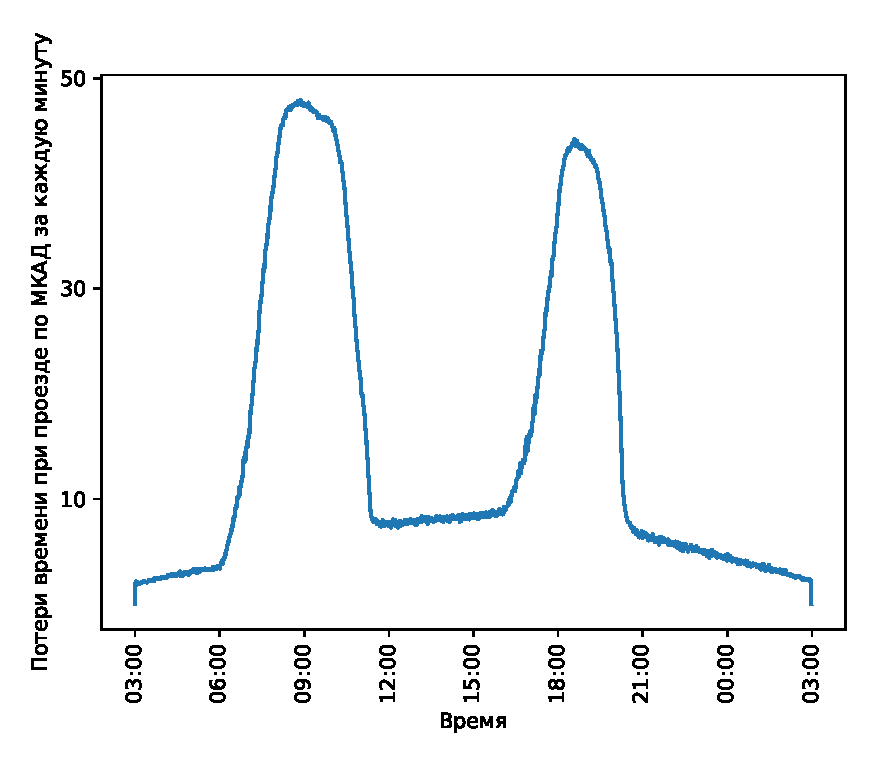
\includegraphics[width=1\linewidth]{MCAR_full_woenters_12_two_types_110_24h_3h_fullFD_handcontrol_Time_to_pass.eps}
        \caption{Временные потери на проезд по автомагистрали в эксперименте с высокой загрузкой с управлением въездами с расчетом всех фундаментальных диаграмм.}
        \label{fig:MCAR_timeloss_hight_3h_handcontrol_FD}
    \end{minipage}
\end{figure}

На графиках видно уменьшение времени затора на МКАД, а также небольшое увеличение числа проехавших автомобилей.
Хотя число проехавших по МКАД автомобилей увеличилось незначительно, временные потери на проезд по автомагистрали сильно снизились, а временной интервал затрудненного движения уменьшился.
Интегральная разность между графиками на рис.~\ref{fig:MCAR_timeloss_hight_3h_FD}~и~\ref{fig:MCAR_timeloss_hight_3h_handcontrol_FD} составляет ровно \(14\) минут.


\section{Сравнение с экспериментами с несколькими фундаментальными диаграммами}
Видно, что модель показала свою устойчивость относительно точности расчета фундаментальных диаграмм.
Несмотря на то, что результаты изменились, общая картина формирования и распространения затора в модели МКАД осталась неизменна.

Эксперименты из разделов~\ref{sec:ch5/average} и~\ref{sec:ch6/average_FD} показывают схожую картину МКАД в течении дня.
Однако, ввиду более аккуратных расчетов МКАД при средней загрузке сам по себе оказывается менее нагружен, а заторное состояние наблюдается меньшее время.
Таким образом даже без управления въездами состояние МКАДа удовлетворительно для проезда и преимущества от управления в этом варианте минимальные~--- всего одна минута.

В эксперименте с высокой загрузкой на въездах~\ref{sec:ch6/hight_FD} преимущество от управления все еще существенное~--- \(14\) минут.
Это меньше чем в эксперименте из раздела~\ref{sec:ch5/hight} на \(4\) минуты, но все еще очень существенно.
Тут мы также наблюдаем небольшие изменения в структуре распространения заторов.

Окончательно, для детального моделирования автомагистрали следует использовать как можно больше информации о её стуктуре, что приводит нас к необходимости использования наибольшего числа фундаментальных диаграмм.
Несмотря на то, что общий результат экспериментов схож, это позволит нам не злоупотреблять светофорным управлением в тех ситуациях, когда в этом нет явной необходимости, что показывает нам сравнение экспериментов со средней загрузкой,
а также более детально управлять въездами при сильно загруженности автомагистрали, не перекрывая въезды на те сегменты магистрали которые не являются ключевыми в формировании заторного движения.


\chapter{Сравнение скорости и результатов моделирования с моделью разумного водителя (IDM)}\label{sec:ch7}
Целью данного раздела является демонстрация применимости предложенной математической модели для моделирования больших транспортных сетей за существенно меньшее в сравнении с микроскопическими моделями, на примере модели разумного водителя~\cite{treiber2000congested}, время.
Ввиду того, что модель разумного водителя является одной из классических моделей, проводится сравнение результатов предложенной авторами модели с результатами микроскопической модели, а также показывается значительное преимущество предложенной модели по скорости вычислений.

Сравнение с моделью разумного водителя производится по двум основным причинам.
Первая причина это отсутствие достаточного объема реальных данных с дорожных датчиков на всем протяжении МКАД, что приводит нас к необходимости брать достаточно точную модель с целью сравнения результатов моделирования.
Вторая причина это необходимость в управлении въездами как конечная цель нашего исследования, что приводит нас к существенно разрывному потоку на въездах на автомагистраль который лучше моделируется микроскопическими моделями.

Окончательно проводятся два типа экспериментов: с моделированием небольшого участка автомагистрали полностью на основе данных с дорожных датчиков и моделирование всего МКАД.

\section{Прямой участок автомагистрали}
В данном эксперименте рассматривается моделирование одного дня движения на прямом участке автомагистрали длиной 1500 метров без значительных съездов и въездов.
На вход подаются данные с дорожного датчика расположенного в начале участка, результаты сравниваются с данными дорожного датчика расположенного в конце участка.
Результаты моделирования представлены на рис.~\ref{fig:simple_road}.
\begin{figure}[!ht]
\centering
\begin{minipage}[b]{0.49\textwidth}
    \centering
    a)
    \\ 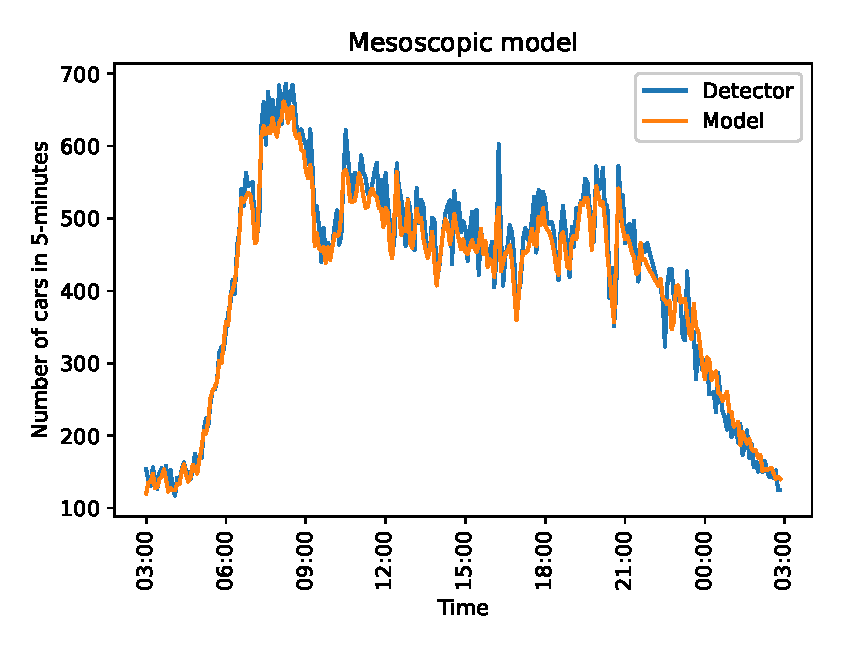
\includegraphics[width=1\linewidth]{simple_road_meso.eps}
\end{minipage}
\hfill
\begin{minipage}[b]{0.49\textwidth}
    \centering
    b)
    \\ 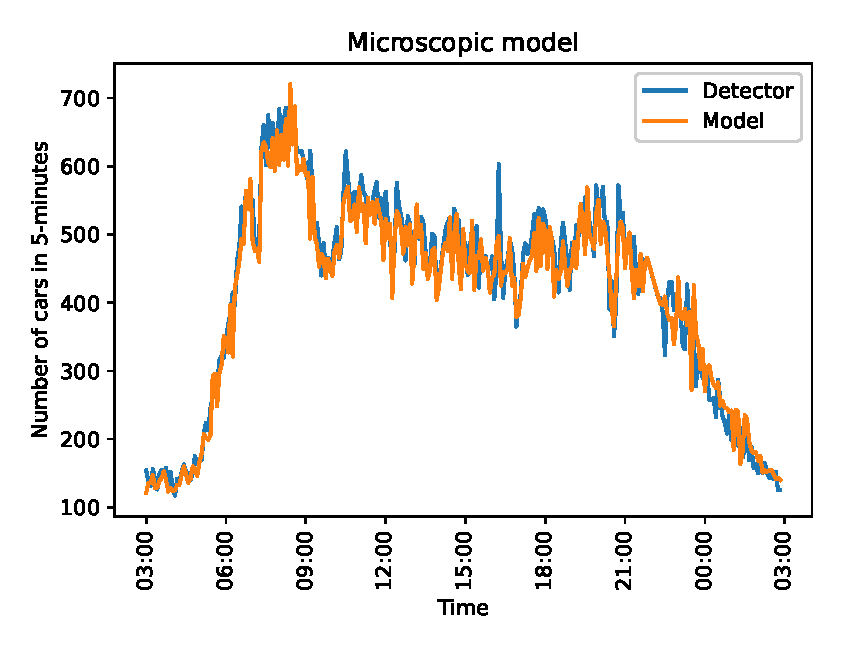
\includegraphics[width=1\linewidth]{simple_road_micro.eps}
\end{minipage}

\caption{а) Результаты моделирования предложенной мезоскопической моделью, b) Результаты моделирования микроскопической моделью.}
\label{fig:simple_road}
\end{figure}
Окончательно, средняя относительная процентная ошибка (mean absolute percentile error - MAPE) для предложенной модели составила 5.35\%, для микроскопической модели составила 5.6\%.
Ошибка предложенной модели относительно модели разумного водителя~- 1.7\%.
Расчётное время на одном ядре CPU мощностью 4.2 ГГц и объёмом оперативной памяти 32 ГБ составило 5.14 секунды для предложенной мезоскопической модели и 88.08 секунд для микроскопической модели.
Значения времени усреднены на основе 100 экспериментов.

Проведем также замеры времени расчётов для обеих подходов при моделировании одного дня прямой дороги с фиксированным потоком АТС на въезде на дорогу в диапазоне от 5 до 48 АТС/мин, а также при фиксированном потоке АТС при увеличении длины моделируемого участка от 500 до 5000 метров.
Результаты экспериментов представлены на рис.~\ref{fig:compare_simple_model}.
Ускорение в моделировании мезоскопической моделью при увеличении числа АТС на въезде связано с групповыми свойствами модели~--- автомобили начали объединяться в группы.
\begin{figure}[!ht]
\centering
\begin{minipage}[b]{0.49\textwidth}
    \centering
    a)
    \\ 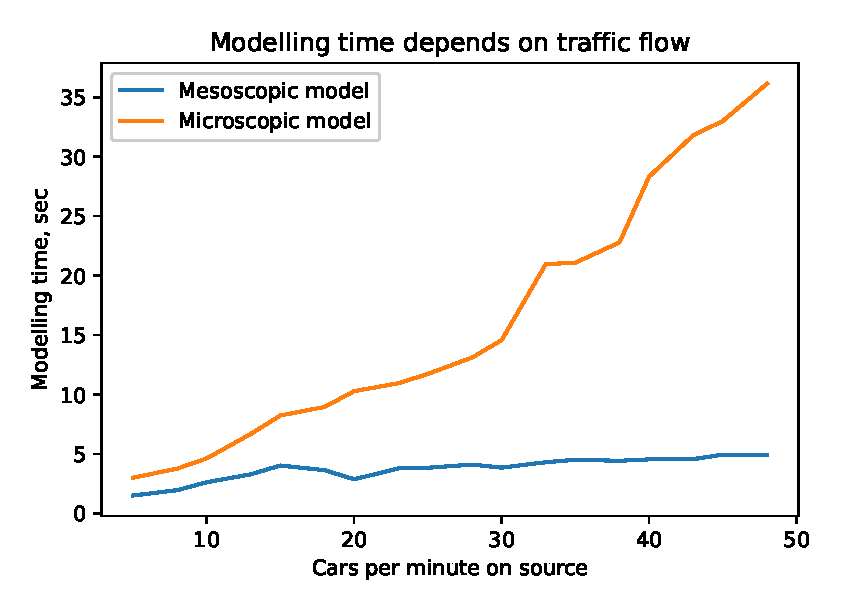
\includegraphics[width=1\linewidth]{modelling_time_cars.eps}
\end{minipage}
\hfill
\begin{minipage}[b]{0.49\textwidth}
    \centering
    b)
    \\ 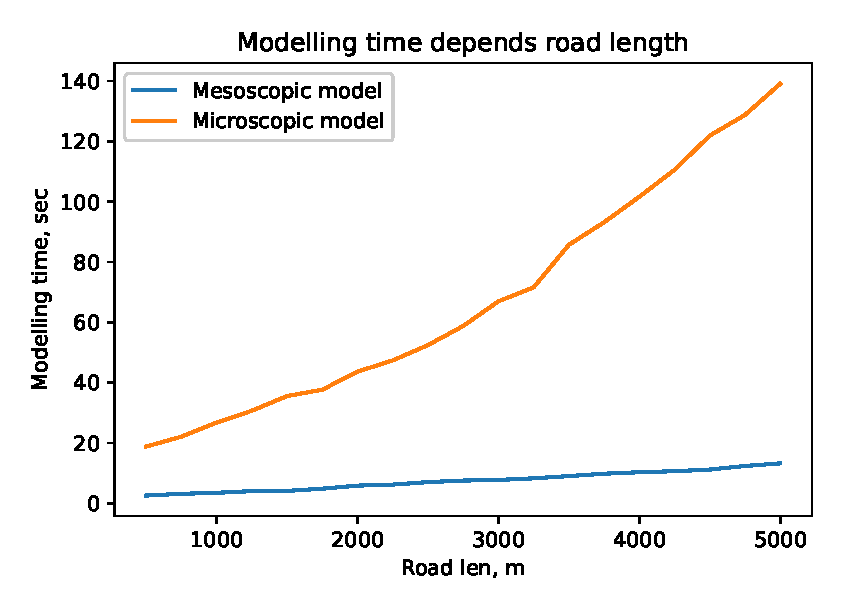
\includegraphics[width=1\linewidth]{modelling_time_length.eps}
\end{minipage}

\caption{а) Время моделирования в зависимости от потока АТС на въезде, b) Время моделирования в зависимости от длины моделируемого участка магистрали при входном потоке 45 АТС/мин.}
\label{fig:compare_simple_model}
\end{figure}


\section{Моделирование всей автомагистрали}
В данном эксперименте проводится моделирование всего МКАД в течении 10 часов, въезды считаются однополосными и функции входного потока изображены на рис.~\ref{fig:MCAR_flow_low_3h}.
В данном случае у нас есть два типа въездов на автомагистраль~--- с утренней и вечерней пиковыми загрузками в течении трёх часов.
\begin{figure}[!ht]
\centering
    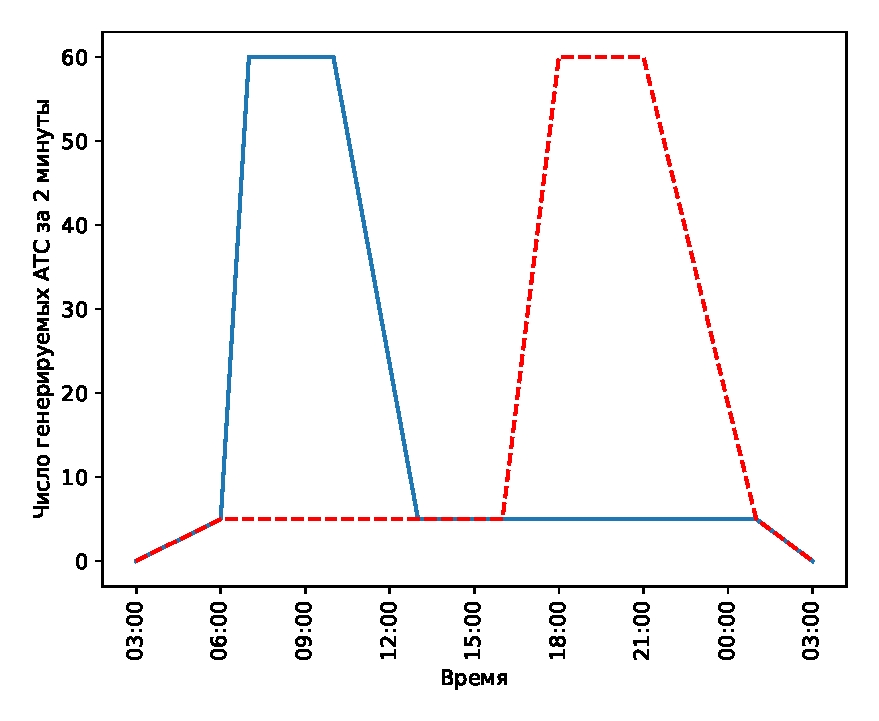
\includegraphics[width=1.0\linewidth]{MCAR_full_woenters_12_two_types_60_24h_3hmax_Enters_generators_idm.eps}
    \caption{Графики загрузки двух типов въездов~--- с утренней и вечерней пиковыми загрузками}
    \label{fig:MCAR_flow_low_3h}
\end{figure}

Результаты моделирования представлены на рис.~\ref{fig:mcar_modelling}
\begin{figure}[!ht]
\centering
\begin{minipage}[b]{0.53\textwidth}
    \centering
    a)
    \\ \includegraphics[width=1\linewidth]{result.eps}
\end{minipage}
\hfill
\begin{minipage}[b]{0.45\textwidth}
    \centering
    b)
    \\ 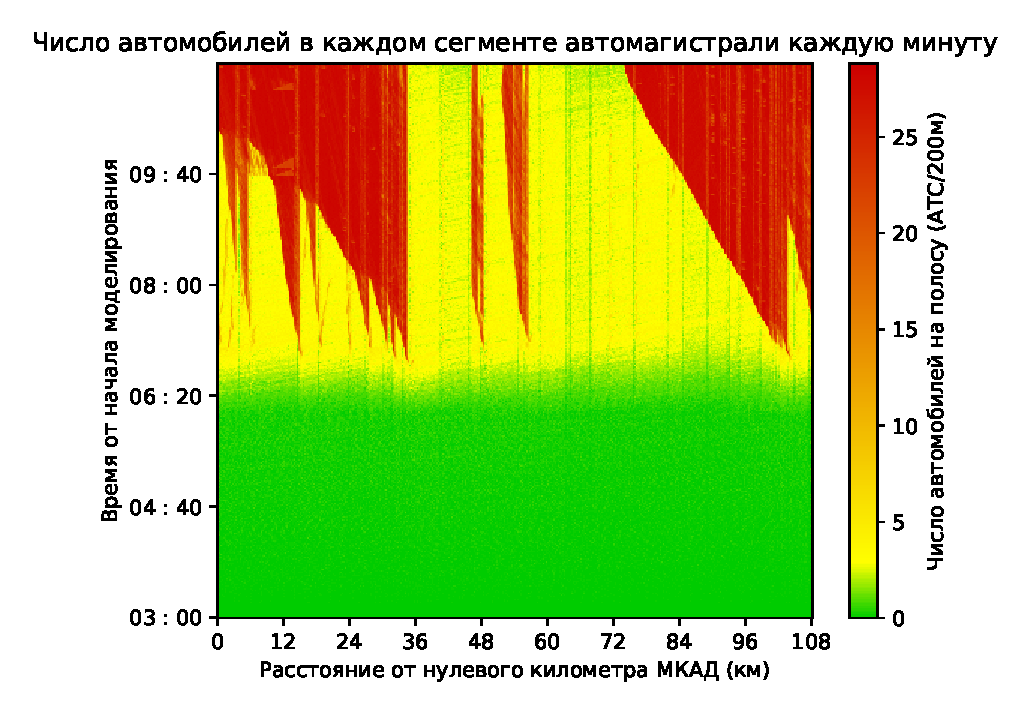
\includegraphics[width=1\linewidth]{MCAR_full_woenters_12_two_types_60_24h_3hmax_fullFD_micro_idm.eps}
\end{minipage}

\caption{а) Результаты моделирования предложенной мезоскопической моделью, b) Результаты моделирования микроскопической моделью.}
\label{fig:mcar_modelling}
\end{figure}
Отметим, что в зоне свободного движения автомобилей, как это видно на рис.~\ref{fig:mcar_modelling}, ошибка достаточно высока ввиду того, что расхождение даже в 1 автомобиль приводит нас к относительной погрешности вплоть до 50\%.
Данная ситуация возникает ввиду того, что микроскопическая модель дискретна на съездах с автомагистрали~--- автомобиль либо полностью съезжает либо полностью остается на магистрали.
Предложенная же мезоскопическая модель не воспринимает число автомобилей в группе как дискретную величину и автомобили в ней съезжают в автомагистрали более равномерно.
При большом потоке автомобилей в среднем мы получаем одинаковое число съехавших транспортных средств, но при малом может наблюдаться существенное расхождение.
Это приводит нас к выводу, что предложенная модель малоприменима для детального моделирования поведения малого числа автомобилей.
Однако, моделирование свободного потока на уровне АТС/минуту не является целью данной модели.
Ввиду данных замечаний расчёт ошибки проводится только для сегментов на которых хотя бы одна из моделей предсказывает поток выше 10 АТС/минуту.

Окончательно, средняя абсолютная процентная ошибка (mean absolute percentile error - MAPE) между предложенной моделью и моделью разумного водителя составила 5.4\%.
Если же рассматривать ошибку определения режима работы автомагистрали, которая интересует нас ввиду того, что мы рассматриваем нашу предложенную модель в первую очередь не для точного определения проехавших автомобилей, а для отслеживания изменения режима работы автомагистрали с целью светофорного управления ею, то ошибка определения режима составит 2.8\%.
Расчет ошибки определения режима проводился следующим образом - число АТС/минуту разделялось на 3 диапазона - от 0 до 10, от 10 до 20, от 20 до 30.
При совпадении предсказанных моделями диапазонов в конкретное время в конкретном сегменте значение ошибки принималось за 0, иначе - за 1.
Окончательно рассчитывается среднее значение ошибки по всем сегментам для всего моделируемого времени.
Расчётное время на одном ядре CPU мощностью 4.2 ГГц и объёмом оперативной памяти 32 ГБ составило 25 минут 26 секунд для предложенной мезоскопической модели и 10 часов 19 минут для микроскопической модели.
Существенное время расчета мезоскопической моделью мы в первую очередь связываем с сильно плотным режимом автомагистрали выбранным для моделирования ввиду наибольшего для нас интереса.

\section{Выводы сравнения с моделью IDM}
Проведено два эксперимента~--- на небольшом участке атомагистрали длиной полтора километра для которого полностью известен поток АТС на обоих его концах на котором можно оценить работоспособность моделей, а также эксперимент с моделированием всего МКАД для оценки временных затрат на моделирование предложенной мезоскопической моделью и классической микроскопической моделью.
Результаты моделирования представлены в таблице~\ref{table:comparsion}.
\begin{table}[htbp]
    \centering
    \caption{Сравнение предложенной модели и модели разумного водителя.\label{table:comparsion}}
    \resizebox{0.85\columnwidth}{!} & 5.6\% & \multicolumn{2}{c|}{5.4\%} \\
    \hline
    \textbf{Время вычислений} & \textbf{5.14 сек} & 88.08 сек & \textbf{25 мин 26 сек} & 10 ч 19 мин \\
    \hline
    \end{tabular}%
    }
 \end{table}
Показано, что предложенная мезоскопическая модель показывает схожие с классическими микроскопическими моделями результаты в рамках как задачи моделирования выделенной автомагистрали так и задачи моделирования участка автомагистрали.
Причём при моделировании участка автомагистрали расчётное время показываемое мезоскопической моделью опережает время микроскопической модели в 17 раз.
При моделировании всего МКАД время расчётов микроскопической моделью оказывается в 24 раза медленнее.
Все вычислительные эксперименты проводились в однопоточном режиме на машине с CPU мощностью 4.2 ГГц и объёмом оперативной памяти 32 ГБ.
Реализация алгоритмов проводилась на языке программирования Python версии 3.11.
Данный результат позволяет использовать мезоскопическую модель в ситуациях когда необходим быстрый результат прогноза при ограниченных вычислительных мощностях.

\clearpage 